\chapter{Аналіз отриманих результатів}
\section{Структурні дані та метод розрахунку}
Як вже було зазначено у вступній частині. Шарувата структура MX$_2$ утворена площинами, що складаються з одного шару атомів M (метал), який знаходиться між двома шарами атомів X (халькоген). Проміжний шар з'єднаний за допомогою сили Ван-дер-Ваальса. Атомна структура шаруватого MX$_2$ показана на рис. \ref{structure} \cite{FU2016221}, (\textbf{b}) показує решітку зверху, підкреслюючи порушення інверсійної симетрії. 

\begin{figure}
	\centering
	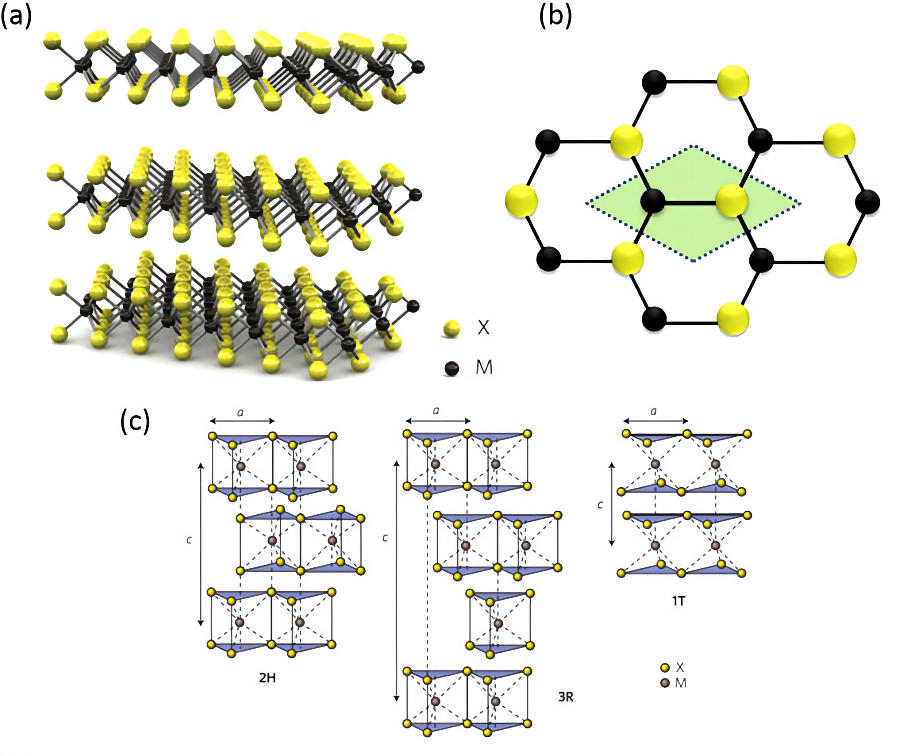
\includegraphics[scale=1]{structure.pdf}
	\caption{(а) тривимірна принципова схема атомної структури шаруватого MX$_2$, атоми металу (M) виділені чорним кольором, а атоми халькогену (X) - жовтим. (b) вид зверху решітки MX$_2$, що підкреслює порушення інверсійної симетрії. (c) схеми структурних політипів. Існує три структурних політипу багатошарової структури MX2: 2H, 3R і 1T з міжшаровим відстанню $\approx$ 0,7 нм.}
	\label{structure}
\end{figure}

У рамках даної роботи вивчалась саме 1T структура. У таблиці \ref{tab:Structure} наведено структурні дані ґратки, які отримані експериментально за допомогою методу рентгенівського дифракційного аналізу.

\begin{table}[!htp]\centering

\scriptsize
\begin{tabular}{lrrrrrrrrrrr}\toprule
\multicolumn{3}{c}{\textbf{TiS$_2$}} & &\multicolumn{3}{c}{\textbf{TiSe$_2$}} & &\multicolumn{3}{c}{\textbf{TiTe$_2$}} \\\midrule
\textbf{a} &\textbf{b} &\textbf{c} & &\textbf{a} &\textbf{b} &\textbf{c} & &\textbf{a} &\textbf{b} &\textbf{c} \\
3.407000 &3.407000 &5.695000 & &3.540000 &3.540000 &6.010000 & &3.768000 &3.768000 &6.460000 \\
\textbf{$\alpha$} &\textbf{$\beta$} &\textbf{$\gamma$} & &\textbf{$\alpha$} &\textbf{$\beta$} &\textbf{$\gamma$} & &\textbf{$\alpha$} &\textbf{$\beta$} &\textbf{$\gamma$} \\
90.000000 &90.000000 &119.999996 & &90.000000 &90.000000 &119.999999 & &90.000000 &90.000000 &119.999998 \\
\textbf{x} &\textbf{y} &\textbf{z} & &\textbf{x} &\textbf{y} &\textbf{z} & &\textbf{x} &\textbf{y} &\textbf{z} \\
0.000000 &0.000000 &0.000000 & &0.000000 &0.000000 &0.000000 & &0.000000 &0.000000 &0.000000 \\
0.333330 &0.666670 &0.749900 & &0.333330 &0.666670 &0.250000 & &0.333330 &0.666670 &0.250000 \\
0.666660 &0.333330 &0.250100 & &0.666660 &0.333330 &0.750000 & &0.666660 &0.333330 &0.750000 \\
\bottomrule
\end{tabular}
\caption{Координати атомів, постійні ґраток та кути TiS$_2$, TiSe$_2$, TiTe$_2$.}\label{tab:Structure}
\end{table}

Розрахунок робився за допомогою програмного пакету VASP (Vienna Ab initio Simulation Package) \cite{VASP1,VASP2, VASP3, VASP4} з PAW методом. Енергія плоских хвиль була в межах до 400 eV та 24 $\times$ 24 $\times$ 12 для розрахунку DOS. Для зонного розрахунку використовувались ті самі значення енергій для плоских хвиль та наступний к-шлях: $\Gamma-M-K-\Gamma-A-L-H-A$.
Вся постоброка відбувалась за допомогою Python 3 \cite{Python} та бібліотек для аналізу DFT розрахунків Pymatgen \cite{PyMatgen}, IFermi \cite{Ifermi}. 

В цілому електронна будова TiS$_2$, TiTe$_2$ та TiSe$_2$ має схожий вигляд. Зона провідності складається з $d$ орбіталей металу, а верх валентної зони складається з $p$ орбіталей і вони перетинаються у точці $L$ для TiS$_2$, $L$ та $M$ у TiSe$_2$, TiTe$_2$. 

Методологія була наступною, спочатку були отримані дані за допомогою звичайного GGA функціоналу у PBE параметризації для порівняння зі SCAN-ом, а саме, наскільки SCAN більш адекватно описує матеріал після структурної релаксації таб. \ref{tab:GGAlat}, таб. \ref{tab:SCANlat}. Та остаточно визначити щілину додавши поправки rVV10, які беруть до уваги взаємодію ван-дер-Ваальса.

\begin{table}[!htp]\centering
\scriptsize
\begin{tabular}{lrrrrrrr}\toprule
\multicolumn{7}{c}{\textbf{GGA}} \\\midrule
\multicolumn{3}{c}{\textbf{Оптимізована струкута}} & &\multicolumn{3}{c}{\textbf{\%}} \\
\multicolumn{7}{c}{\textbf{TiS$_2$}} \\
\textbf{a} &\textbf{b} &\textbf{c} & &\textbf{a} &\textbf{b} &\textbf{c} \\
3.412015 &3.412013 &6.446000 & &0.147089 &0.147030 &12.371304 \\
\textbf{$\alpha$} &\textbf{$\beta$} &\textbf{$\gamma$} & &\textbf{$\alpha$} &\textbf{$\beta$} &\textbf{$\gamma$} \\
89.999997 &90.000022 &119.999994 & &-0.000003 &0.000024 &-0.000002 \\
\multicolumn{7}{c}{\textbf{TiSe$_2$}} \\
\textbf{a} &\textbf{b} &\textbf{c} & &\textbf{a} &\textbf{b} &\textbf{c} \\
3.541846 &3.541879 &6.603517 & &0.052133 &0.053065 &9.410809 \\
\textbf{$\alpha$} &\textbf{$\beta$} &\textbf{$\gamma$} & &\textbf{$\alpha$} &\textbf{$\beta$} &\textbf{$\gamma$} \\
89.998535 &90.000481 &119.999714 & &-0.001628 &0.000534 &-0.000238 \\
\multicolumn{7}{c}{\textbf{TiTe$_2$}} \\
\textbf{a} &\textbf{b} &\textbf{c} & &\textbf{a} &\textbf{b} &\textbf{c} \\
3.766554 &3.766586 &6.865603 & &-0.038383 &-0.037534 &6.087574 \\
\textbf{$\alpha$} &\textbf{$\beta$} &\textbf{$\gamma$} & &\textbf{$\alpha$} &\textbf{$\beta$} &\textbf{$\gamma$} \\
89.998136 &90.001023 &119.998697 & &-0.002071 &0.001137 &-0.001084 \\
\bottomrule
\end{tabular}
\caption{Відхилення оптимізованої структури від експериментальної за допомогою GGA.}\label{tab:GGAlat}
\end{table}


\begin{table}[!htp]\centering
\scriptsize
\begin{tabular}{lrrrrrrr}\toprule
\multicolumn{7}{c}{\textbf{SCAN}} \\\midrule
\multicolumn{3}{c}{\textbf{Оптимізована струкута}} & &\multicolumn{3}{c}{\textbf{\%}} \\
\multicolumn{7}{c}{\textbf{TiS$_2$}} \\
\textbf{a} &\textbf{b} &\textbf{c} & &\textbf{a} &\textbf{b} &\textbf{c} \\
3.421272 &3.421262 &5.890012 & &0.418027 &0.417734 &3.366626 \\
\textbf{$\alpha$} &\textbf{$\beta$} &\textbf{$\gamma$} & &\textbf{$\alpha$} &\textbf{$\beta$} &\textbf{$\gamma$} \\
90.003098 &89.996423 &120.010782 & &0.003442 &-0.003975 &0.008988 \\
\multicolumn{7}{c}{\textbf{TiSe$_2$}} \\
\textbf{a} &\textbf{b} &\textbf{c} & &\textbf{a} &\textbf{b} &\textbf{c} \\
3.546469 &3.546465 &6.283398 & &0.182573 &0.182461 &4.447883 \\
\textbf{$\alpha$} &\textbf{$\beta$} &\textbf{$\gamma$} & &\textbf{$\alpha$} &\textbf{$\beta$} &\textbf{$\gamma$} \\
90.001939 &89.998709 &119.992066 & &0.002154 &-0.001434 &-0.006611 \\
\multicolumn{7}{c}{\textbf{TiTe$_2$}} \\
\textbf{a} &\textbf{b} &\textbf{c} & &\textbf{a} &\textbf{b} &\textbf{c} \\
3.758144 &3.758125 &6.857830 & &-0.261914 &-0.262419 &5.974397 \\
\textbf{$\alpha$} &\textbf{$\beta$} &\textbf{$\gamma$} & &\textbf{$\alpha$} &\textbf{$\beta$} &\textbf{$\gamma$} \\
89.992373 &90.008670 &119.993283 & &-0.008475 &0.009633 &-0.005596 \\
\bottomrule
\end{tabular}
\caption{Відхилення оптимізованої структури від експериментальної за допомогою SCAN.}\label{tab:SCANlat}
\end{table}

\clearpage
\begin{figure}[H]
\centering
	\begin{subfigure}[b]{.9\textwidth}
    	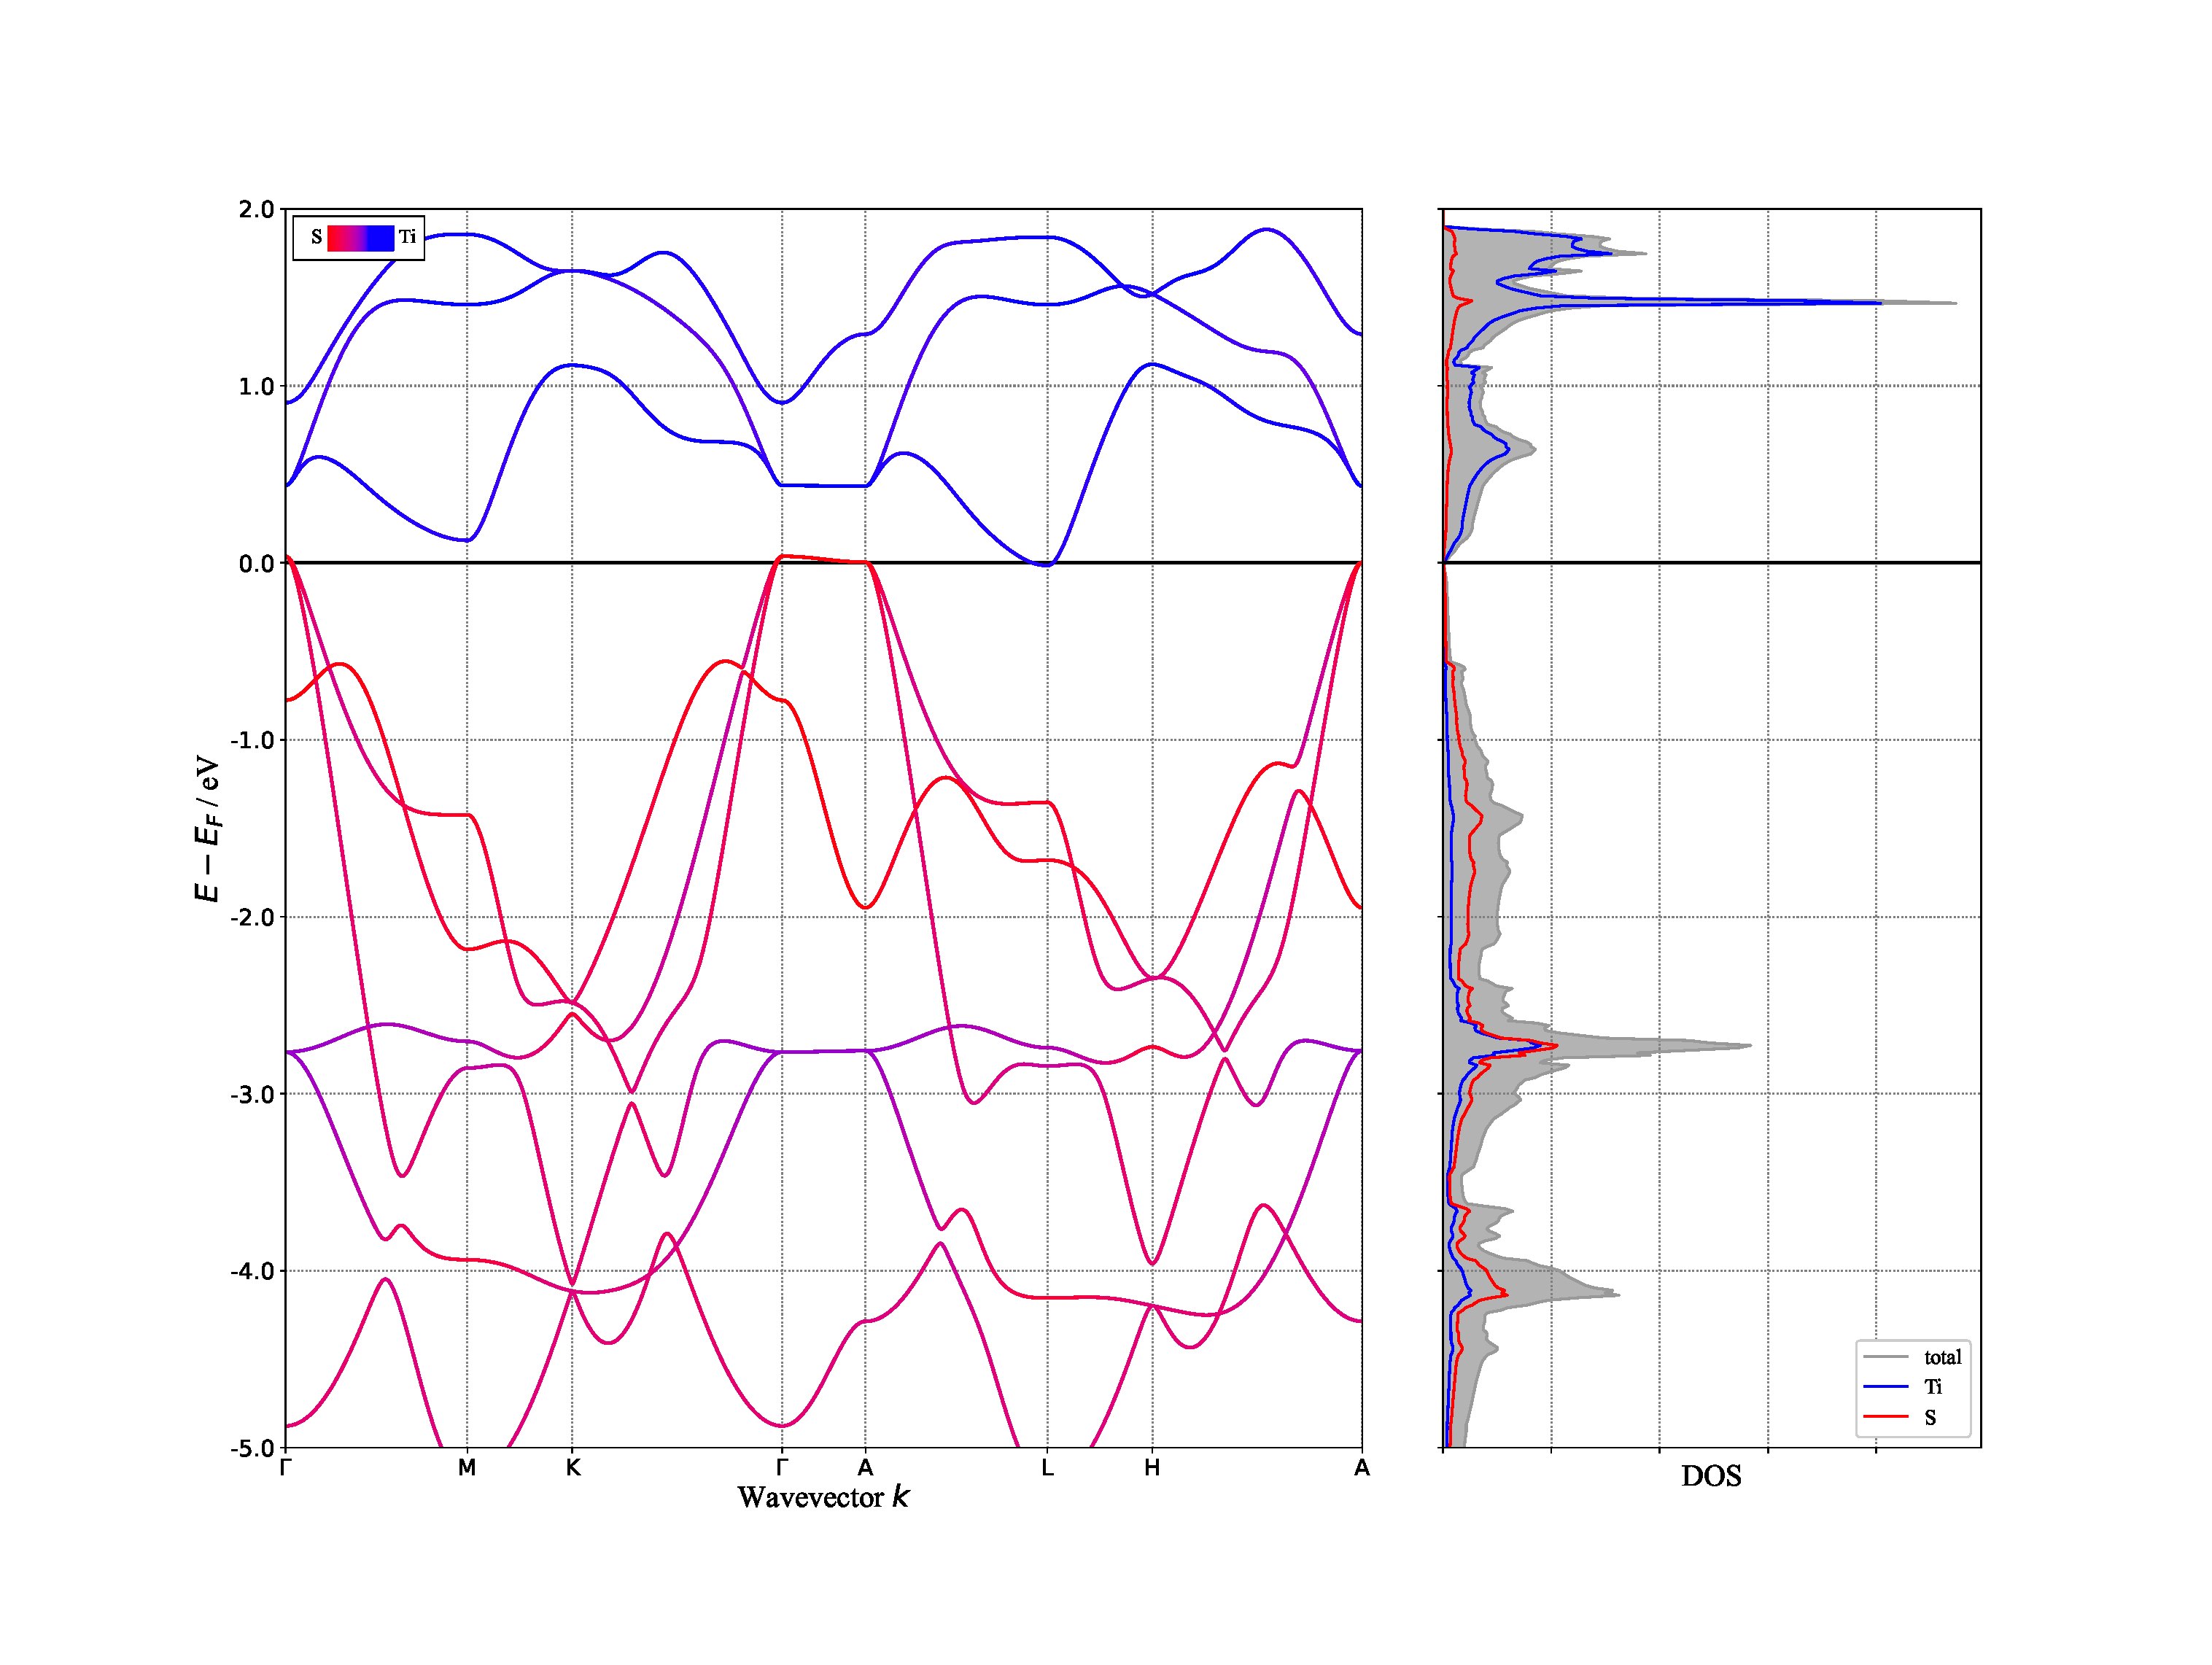
\includegraphics[width=\linewidth]{img/results/TiS2_GGA_relaxed_BAND+DOS.eps}
    	\caption{TiS2}
	\end{subfigure}
	\begin{subfigure}[b]{.4\textwidth}
    	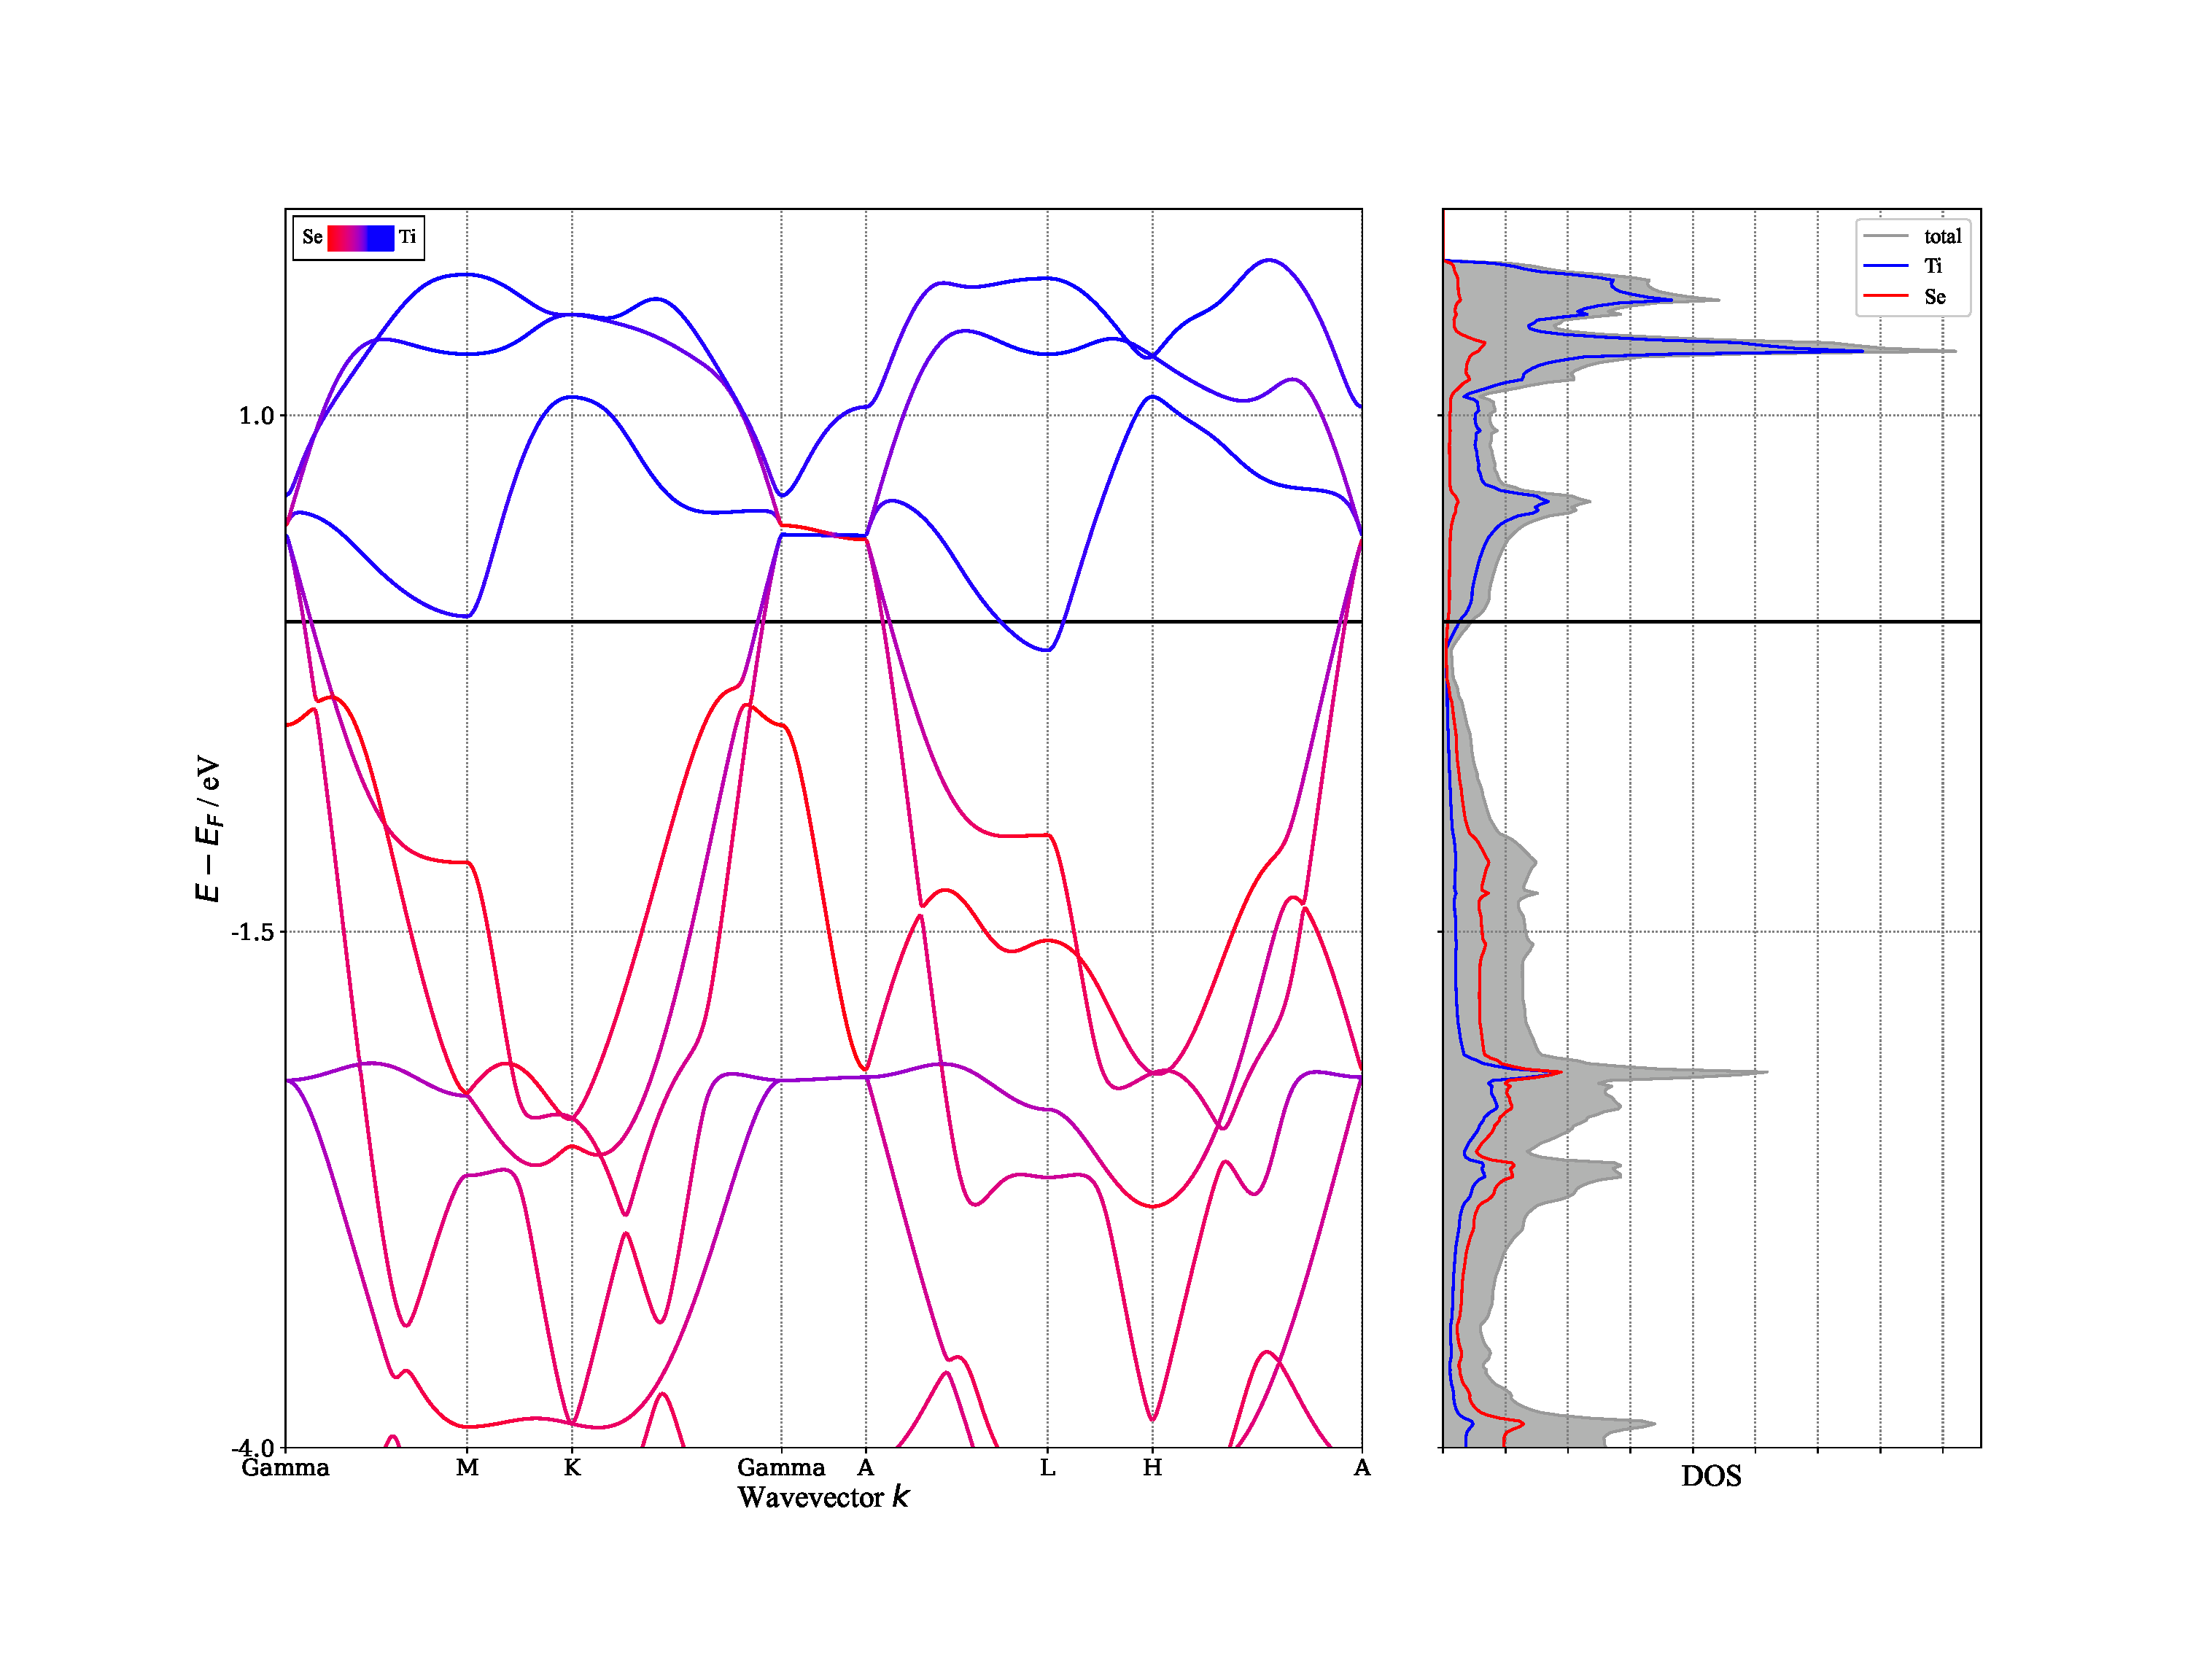
\includegraphics[width=\linewidth]{img/results/TiSe2_GGA_relaxed_BAND+DOS.eps}
    	\caption{
    	TiSe2}
	\end{subfigure}
	\begin{subfigure}[b]{.4\textwidth}
    	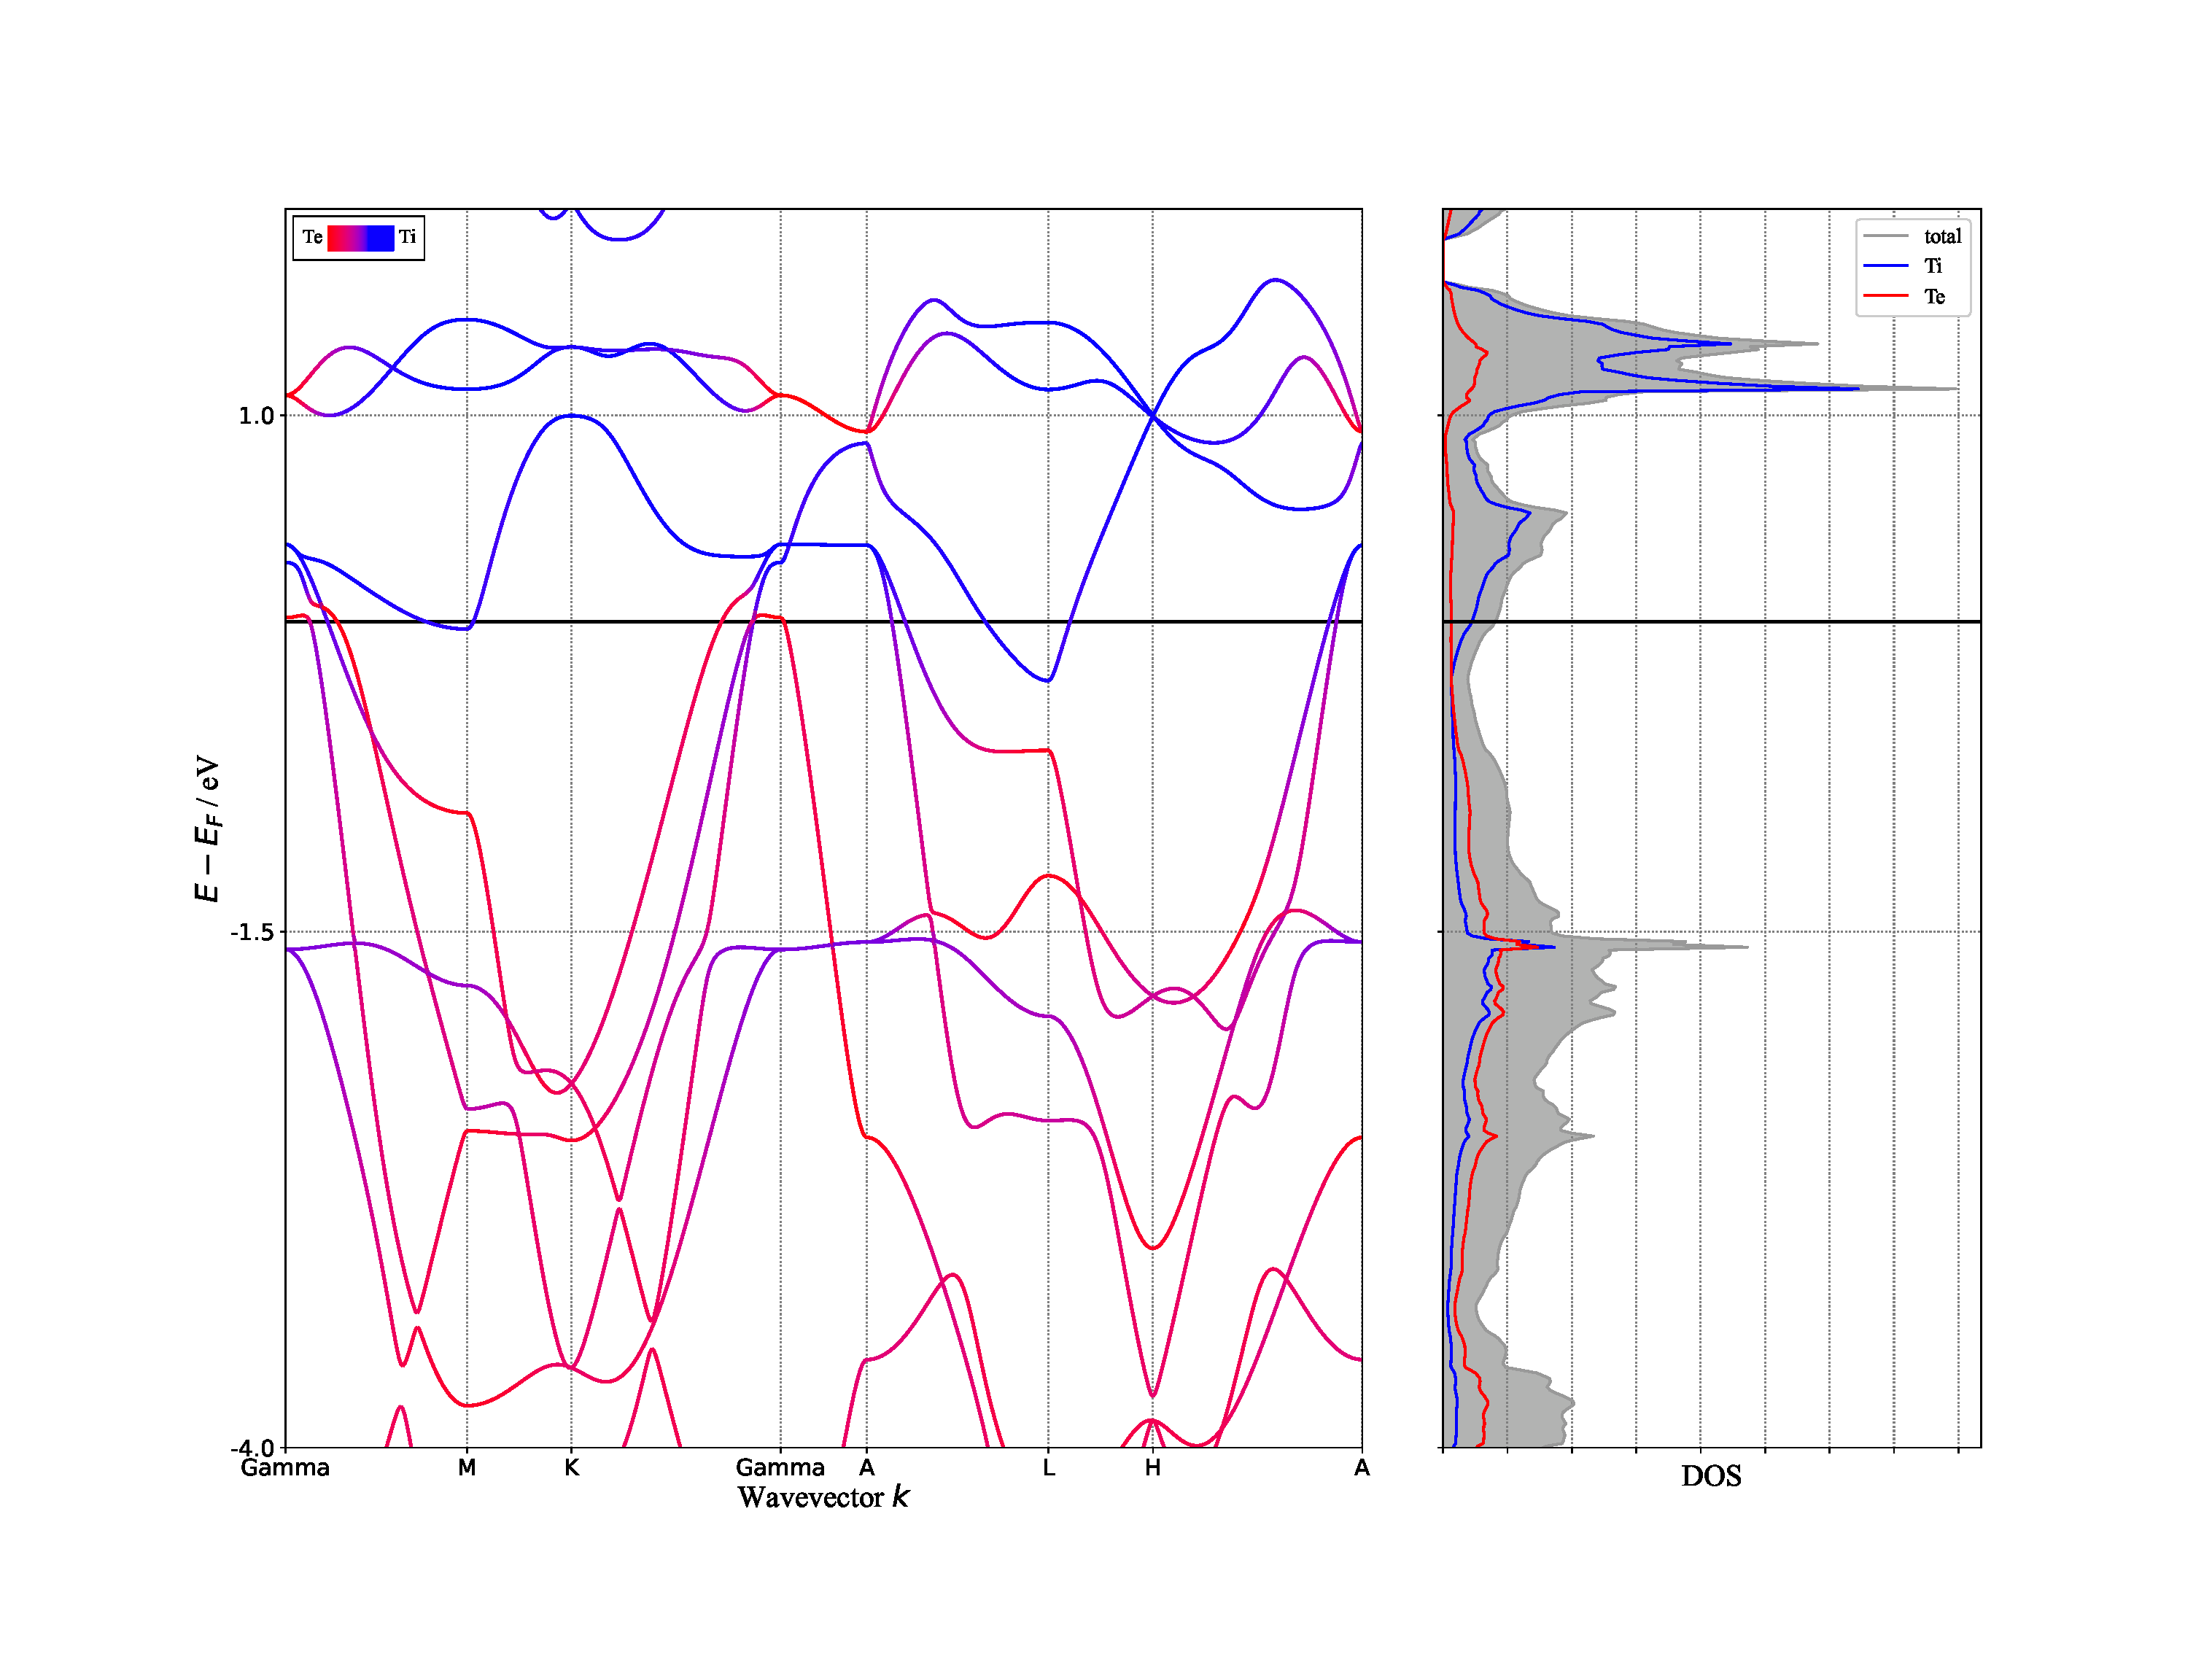
\includegraphics[width=\linewidth]{img/results/TiTe2_GGA_relaxed_BAND+DOS.eps}
    	\caption{
    	TiTe2}
	\end{subfigure}
\caption{Електронна будова TiS$_2$, TiSe$_2$, TiTe$_2$ червоним кольором позначено вклад атомів халькогену (S, Se, Te) синім атомів металу (Ti), розрахована з GGA.}
\label{fig:bandstructireGGA}
\end{figure}

Було визначено що при використані GGA PBE функціоналу, як і очікувалось, відображає зону структуру, що схожа на компенсований метал див. рис. \ref{fig:bandstructireGGA}. На малюнку \ref{fig:fermisurf}, як раз можна побачити, що об'єм електронних карманів приблизно дорівнює об'єму дірок.

\begin{figure}[H]
\centering
	\begin{subfigure}[b]{.4\textwidth}
    	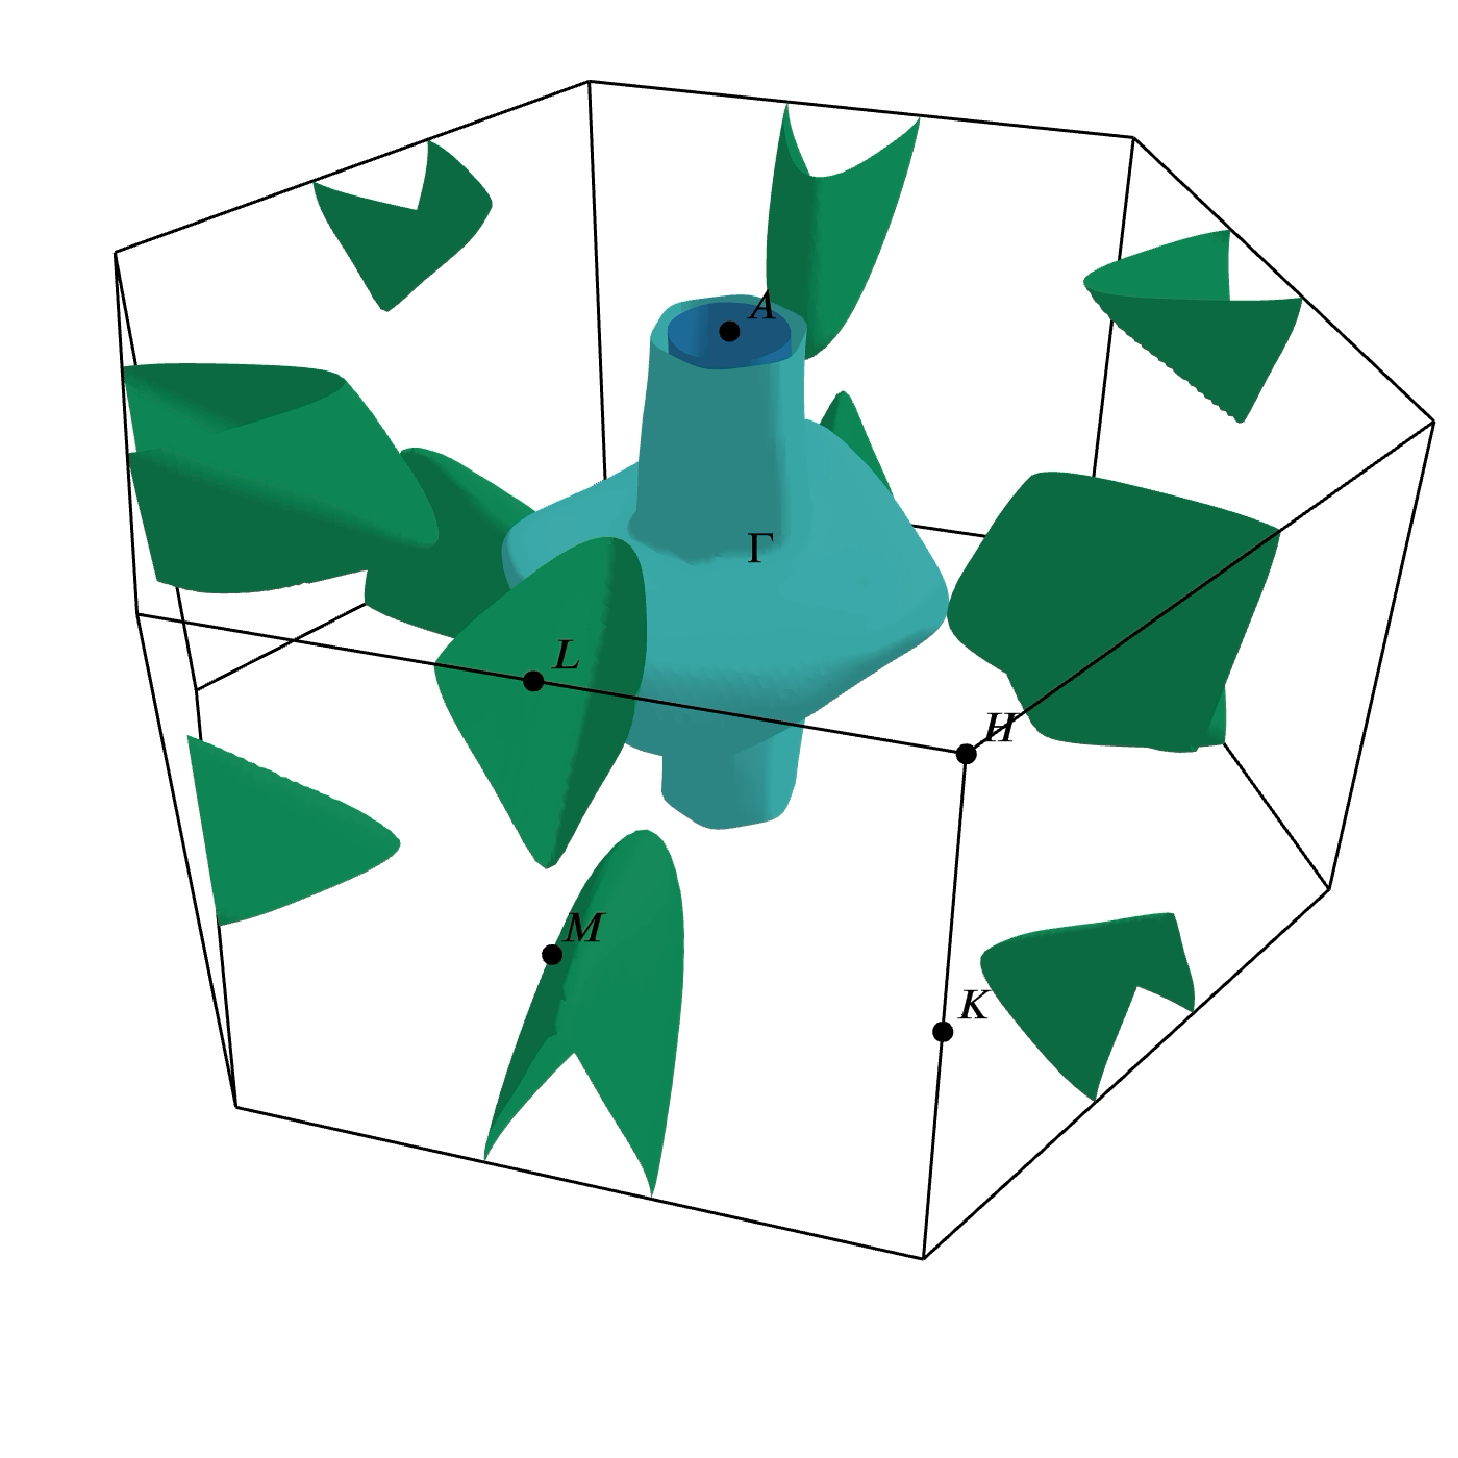
\includegraphics[width=\linewidth]{img/results/fstite2.pdf}
    	\caption{TiTe2}
	\end{subfigure}
	\begin{subfigure}[b]{.4\textwidth}
    	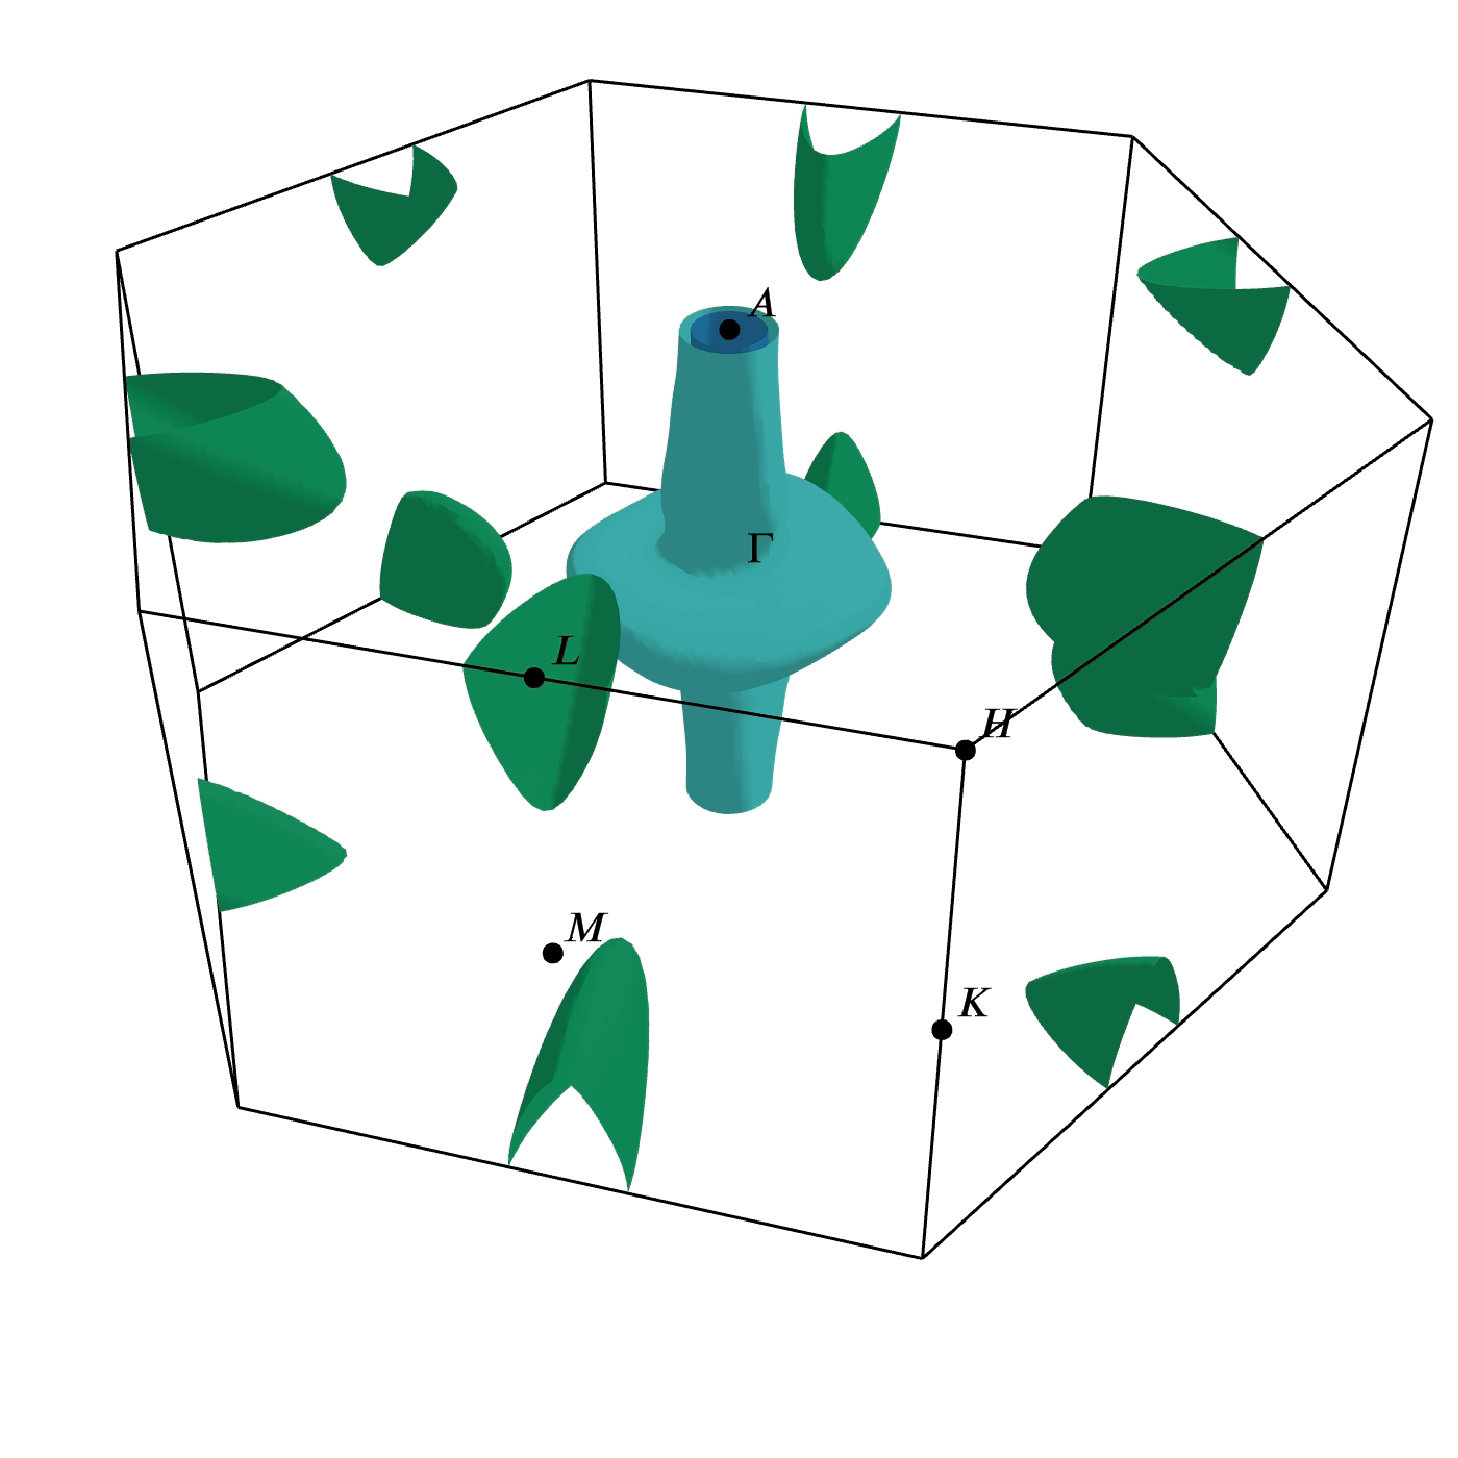
\includegraphics[width=\linewidth]{img/results/fstise2.pdf}
    	\caption{
    	TiSe2}
	\end{subfigure}
	\begin{subfigure}[b]{.9\textwidth}
    	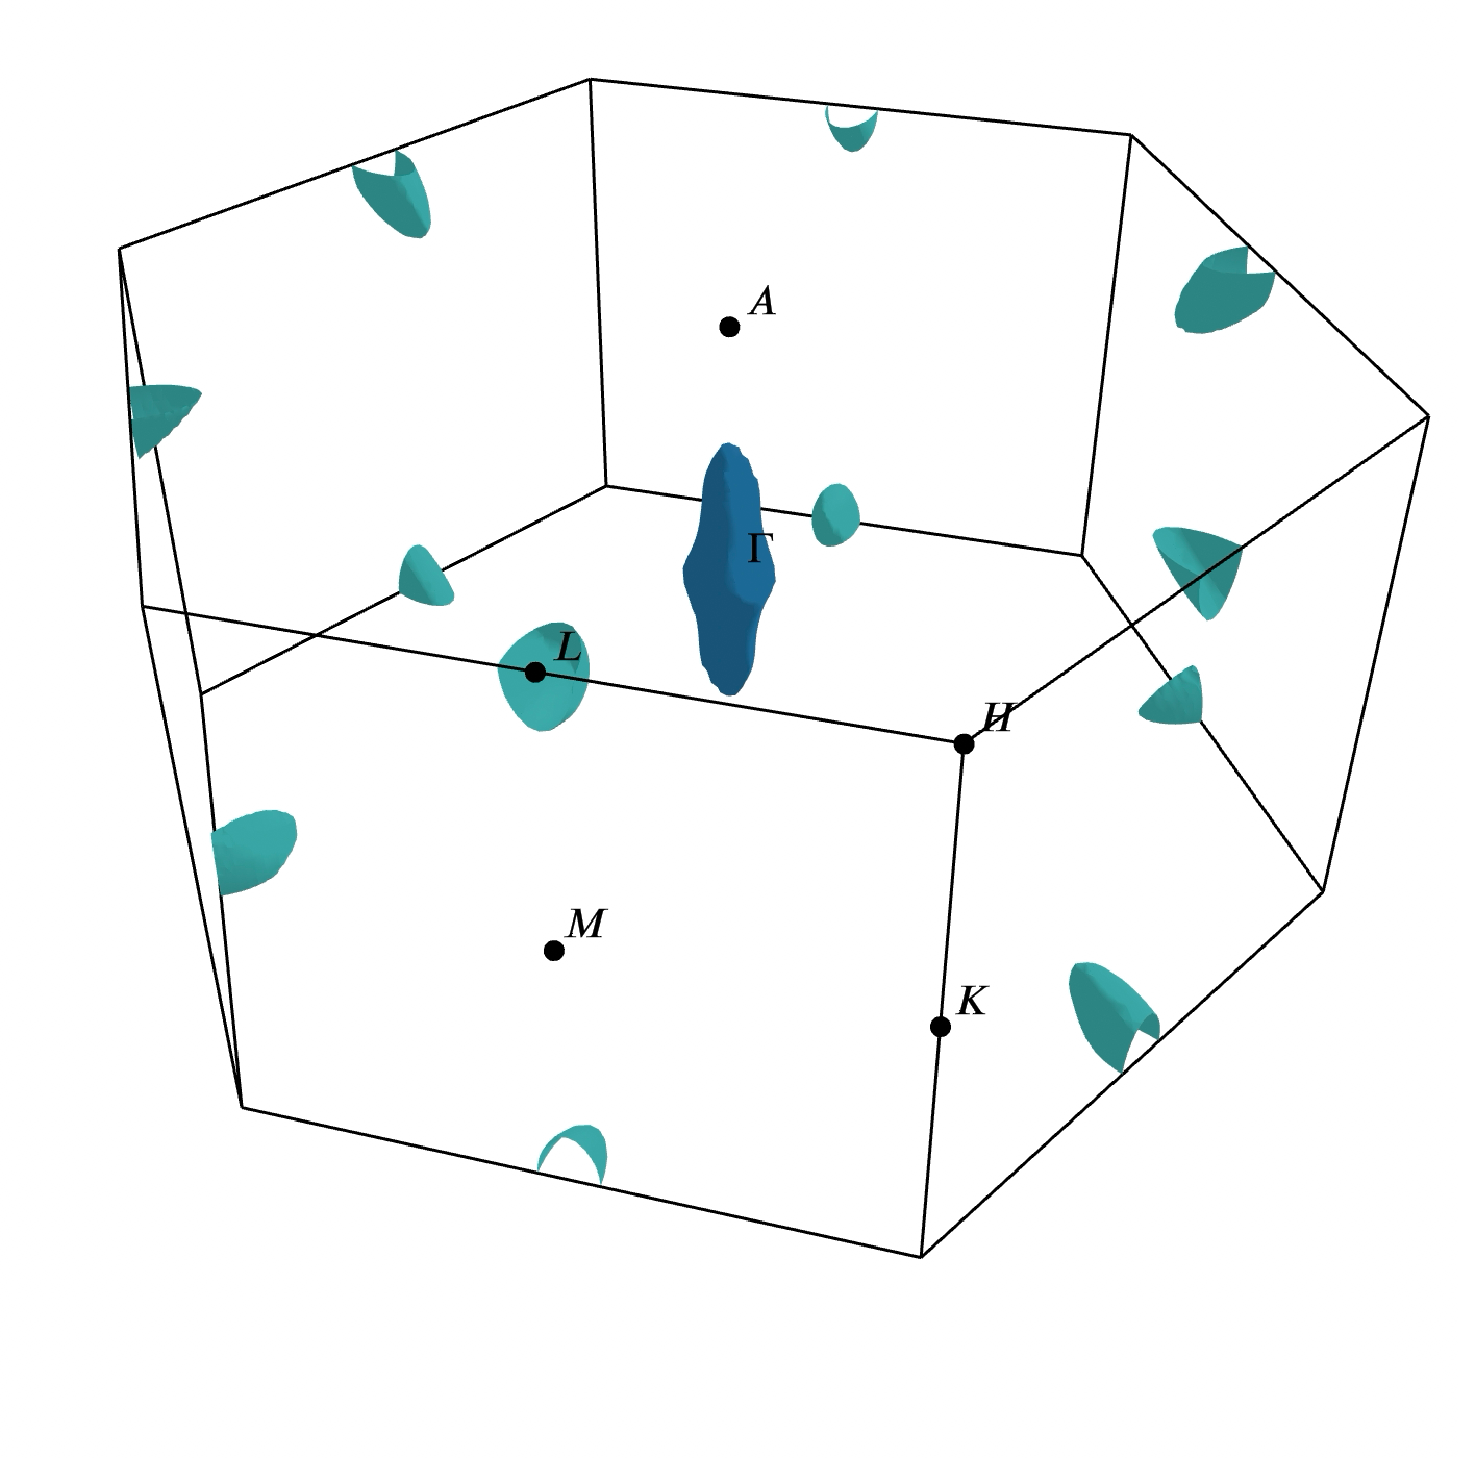
\includegraphics[width=\linewidth]{img/results/fstis2.pdf}
    	\caption{
    	TiS2}
	\end{subfigure}
\caption{Розрахована поверхня фермі TiS$_2$, TiSe$_2$, TiTe$_2$ за допомогою PBE GGA функціоналу.}
\label{fig:fermisurf}
\end{figure}

Після цього було задіяно SCAN функціонал та отримано наступні результати див. мал. \ref{fig:bandstructireSCAN}. Зоні спектри дуже схожі які були розраховані у GGA PBE наближені. Але все ж завдяки тому що SCAN більш точно описує електронну будову ван-дер-Ваальсових матеріалів. То все ж таки перекриття у точці $L$ значно зменшується та становить вже -0.0286 еВ. в $\approx$ 2 менше в порівняні з -0.0633 еВ у GGA PBE. 

\begin{figure}[H]
\centering
	\begin{subfigure}[b]{.9\textwidth}
    	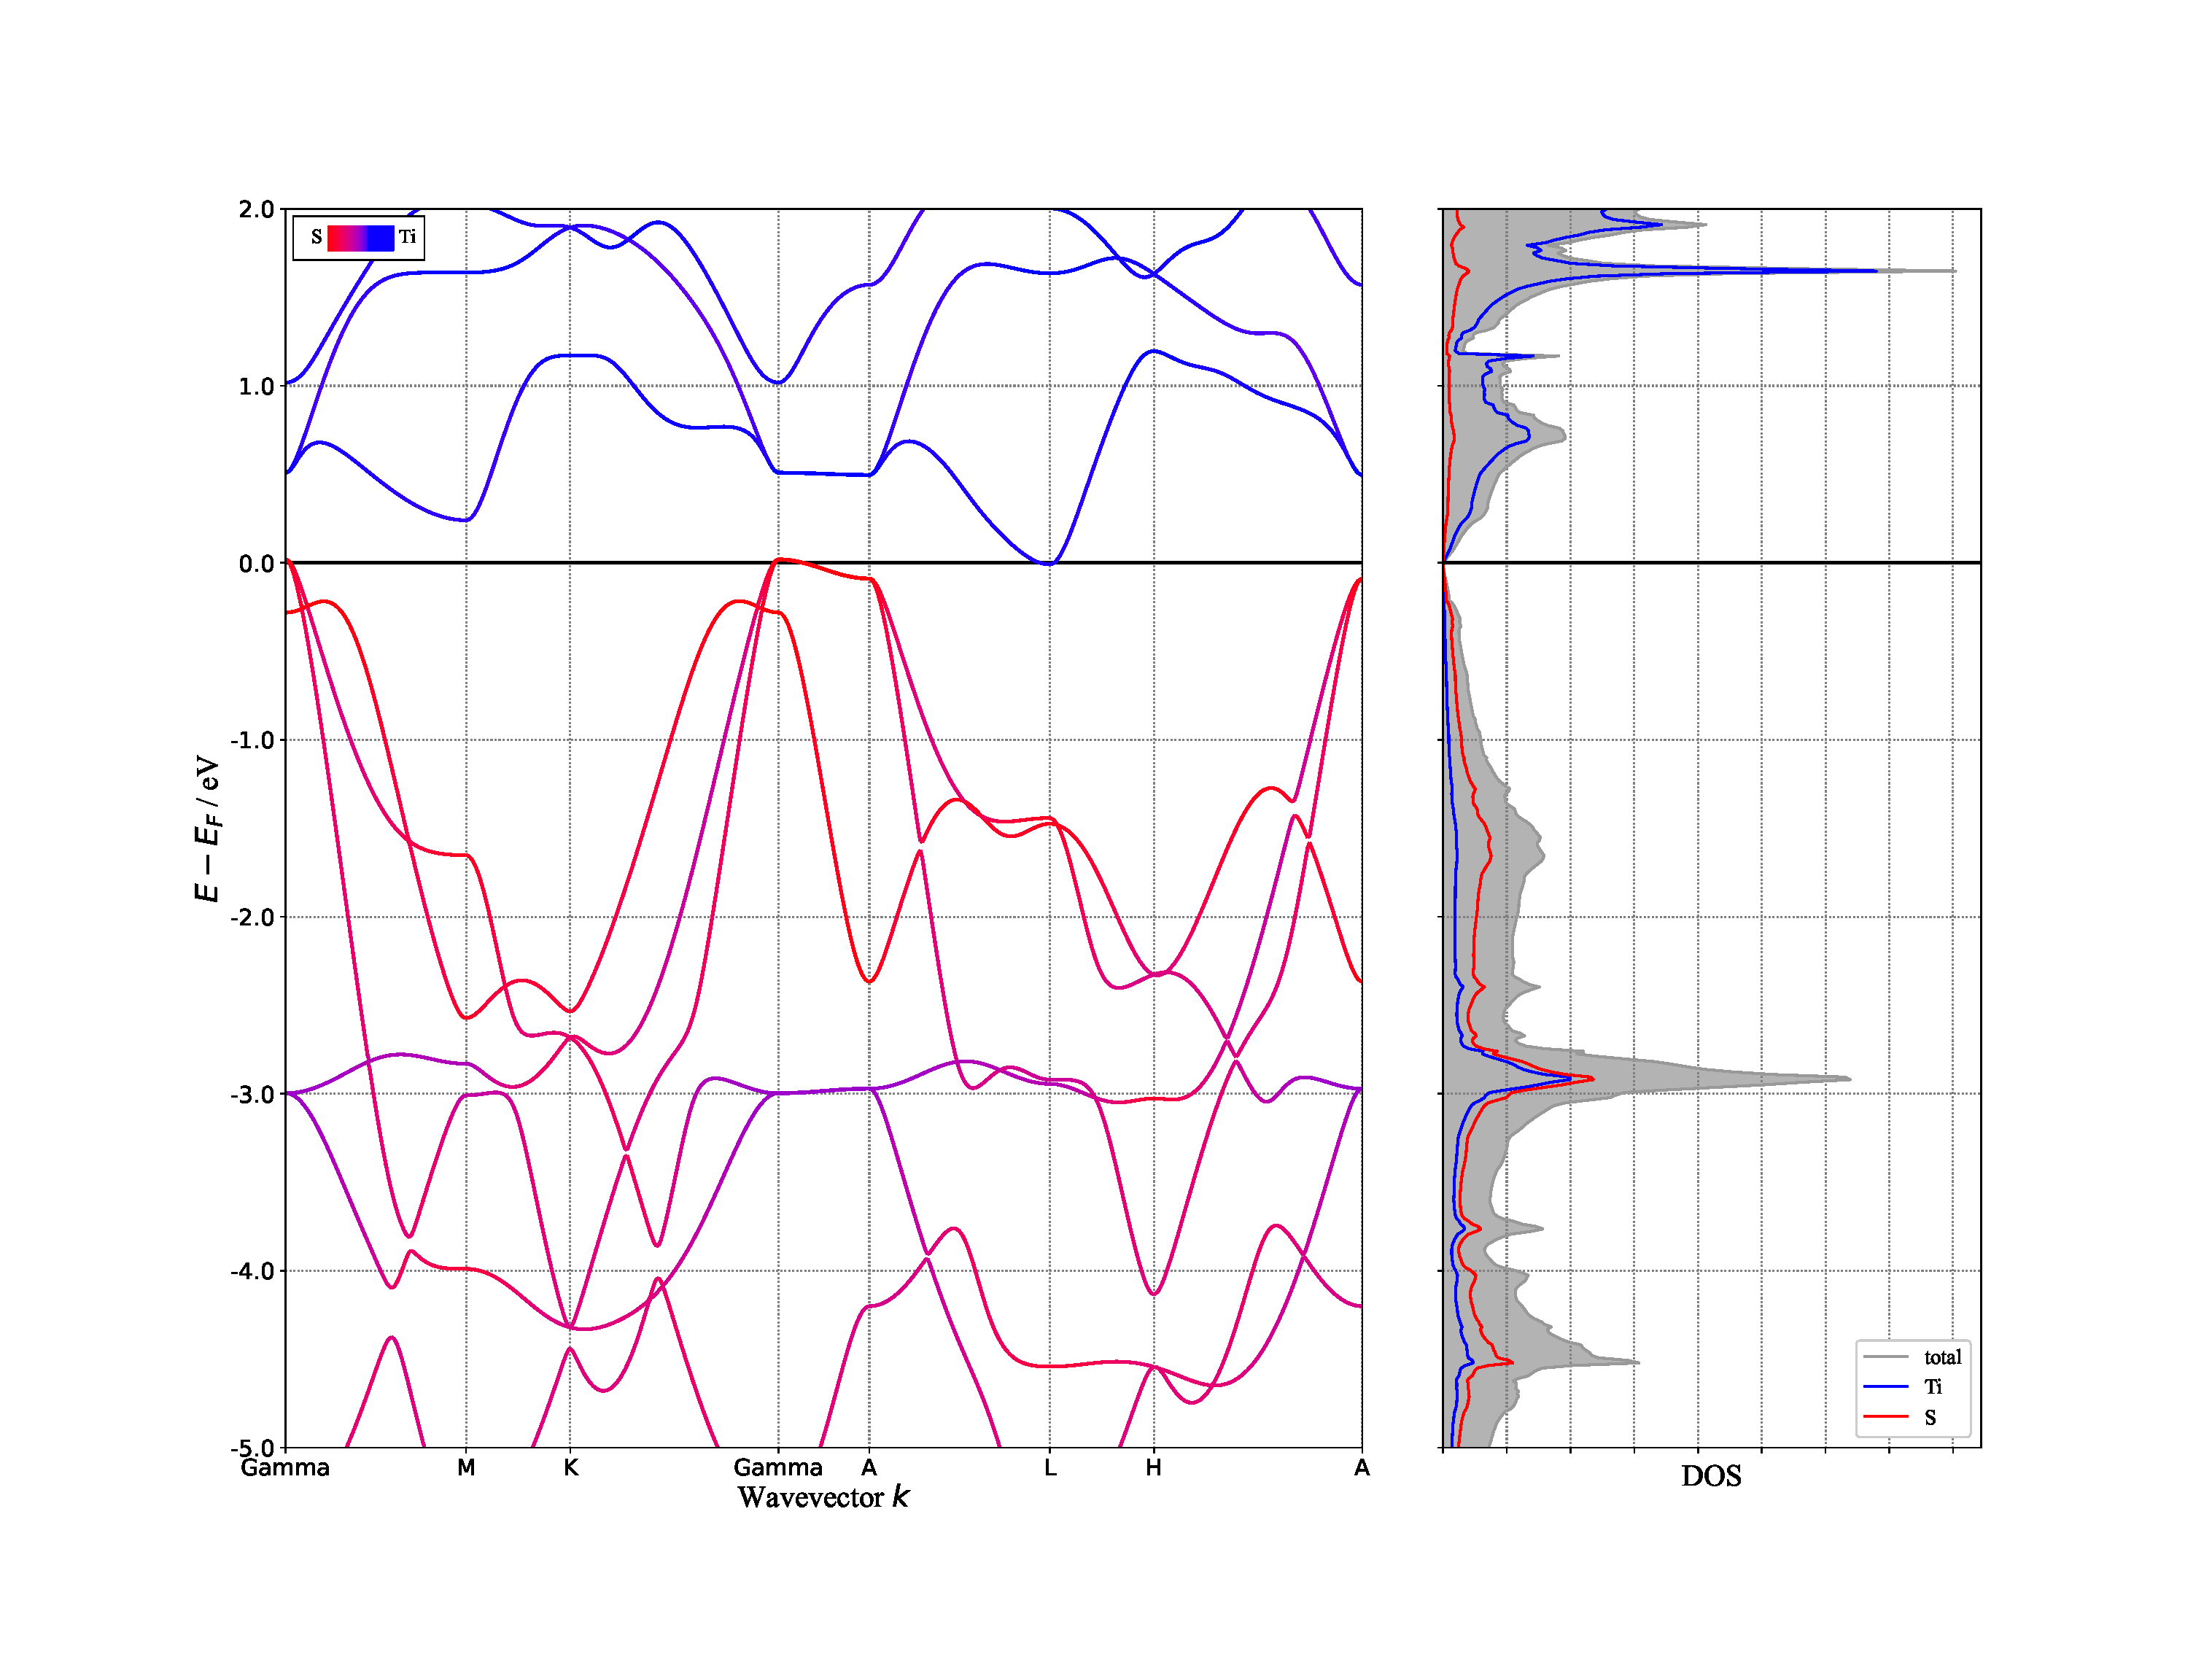
\includegraphics[width=\linewidth]{img/results/TiS2_SCAN_relaxed_BAND+DOS.eps}
    	\caption{TiS2}
	\end{subfigure}
	\begin{subfigure}[b]{.4\textwidth}
    	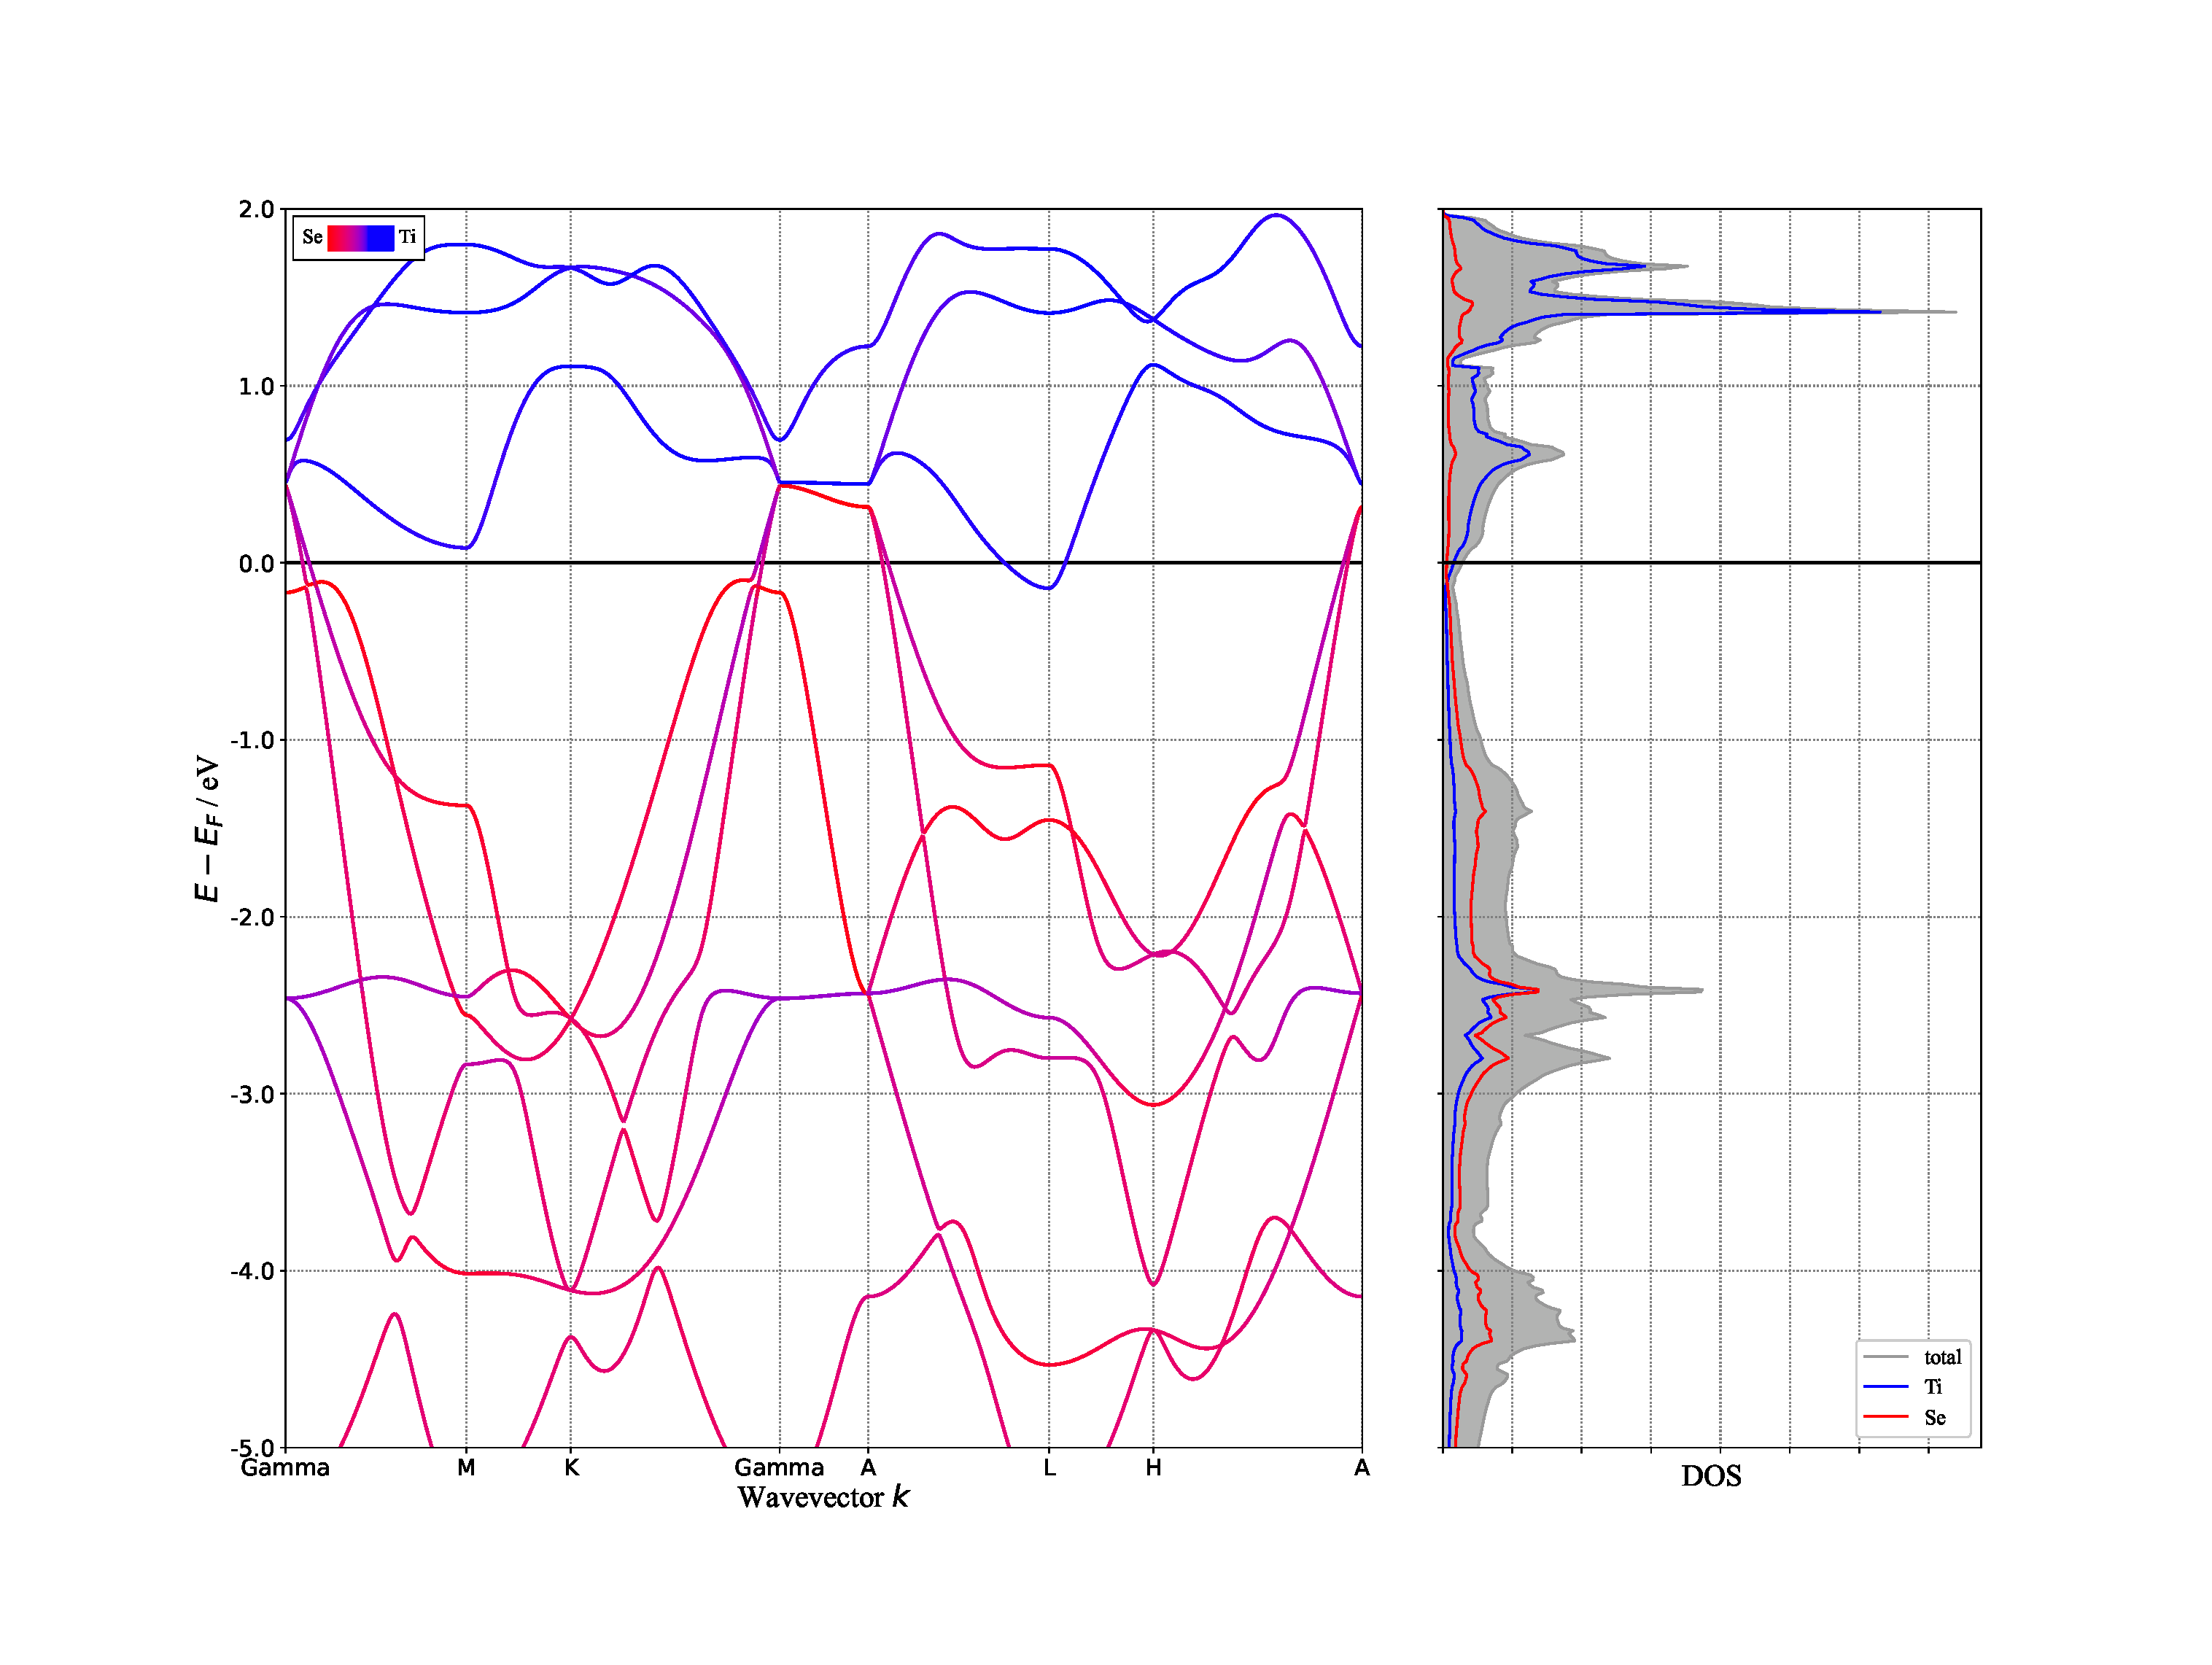
\includegraphics[width=\linewidth]{img/results/TiSe2_SCAN_relaxed_BAND+DOS}
    	\caption{
    	TiSe2}
	\end{subfigure}
	\begin{subfigure}[b]{.4\textwidth}
    	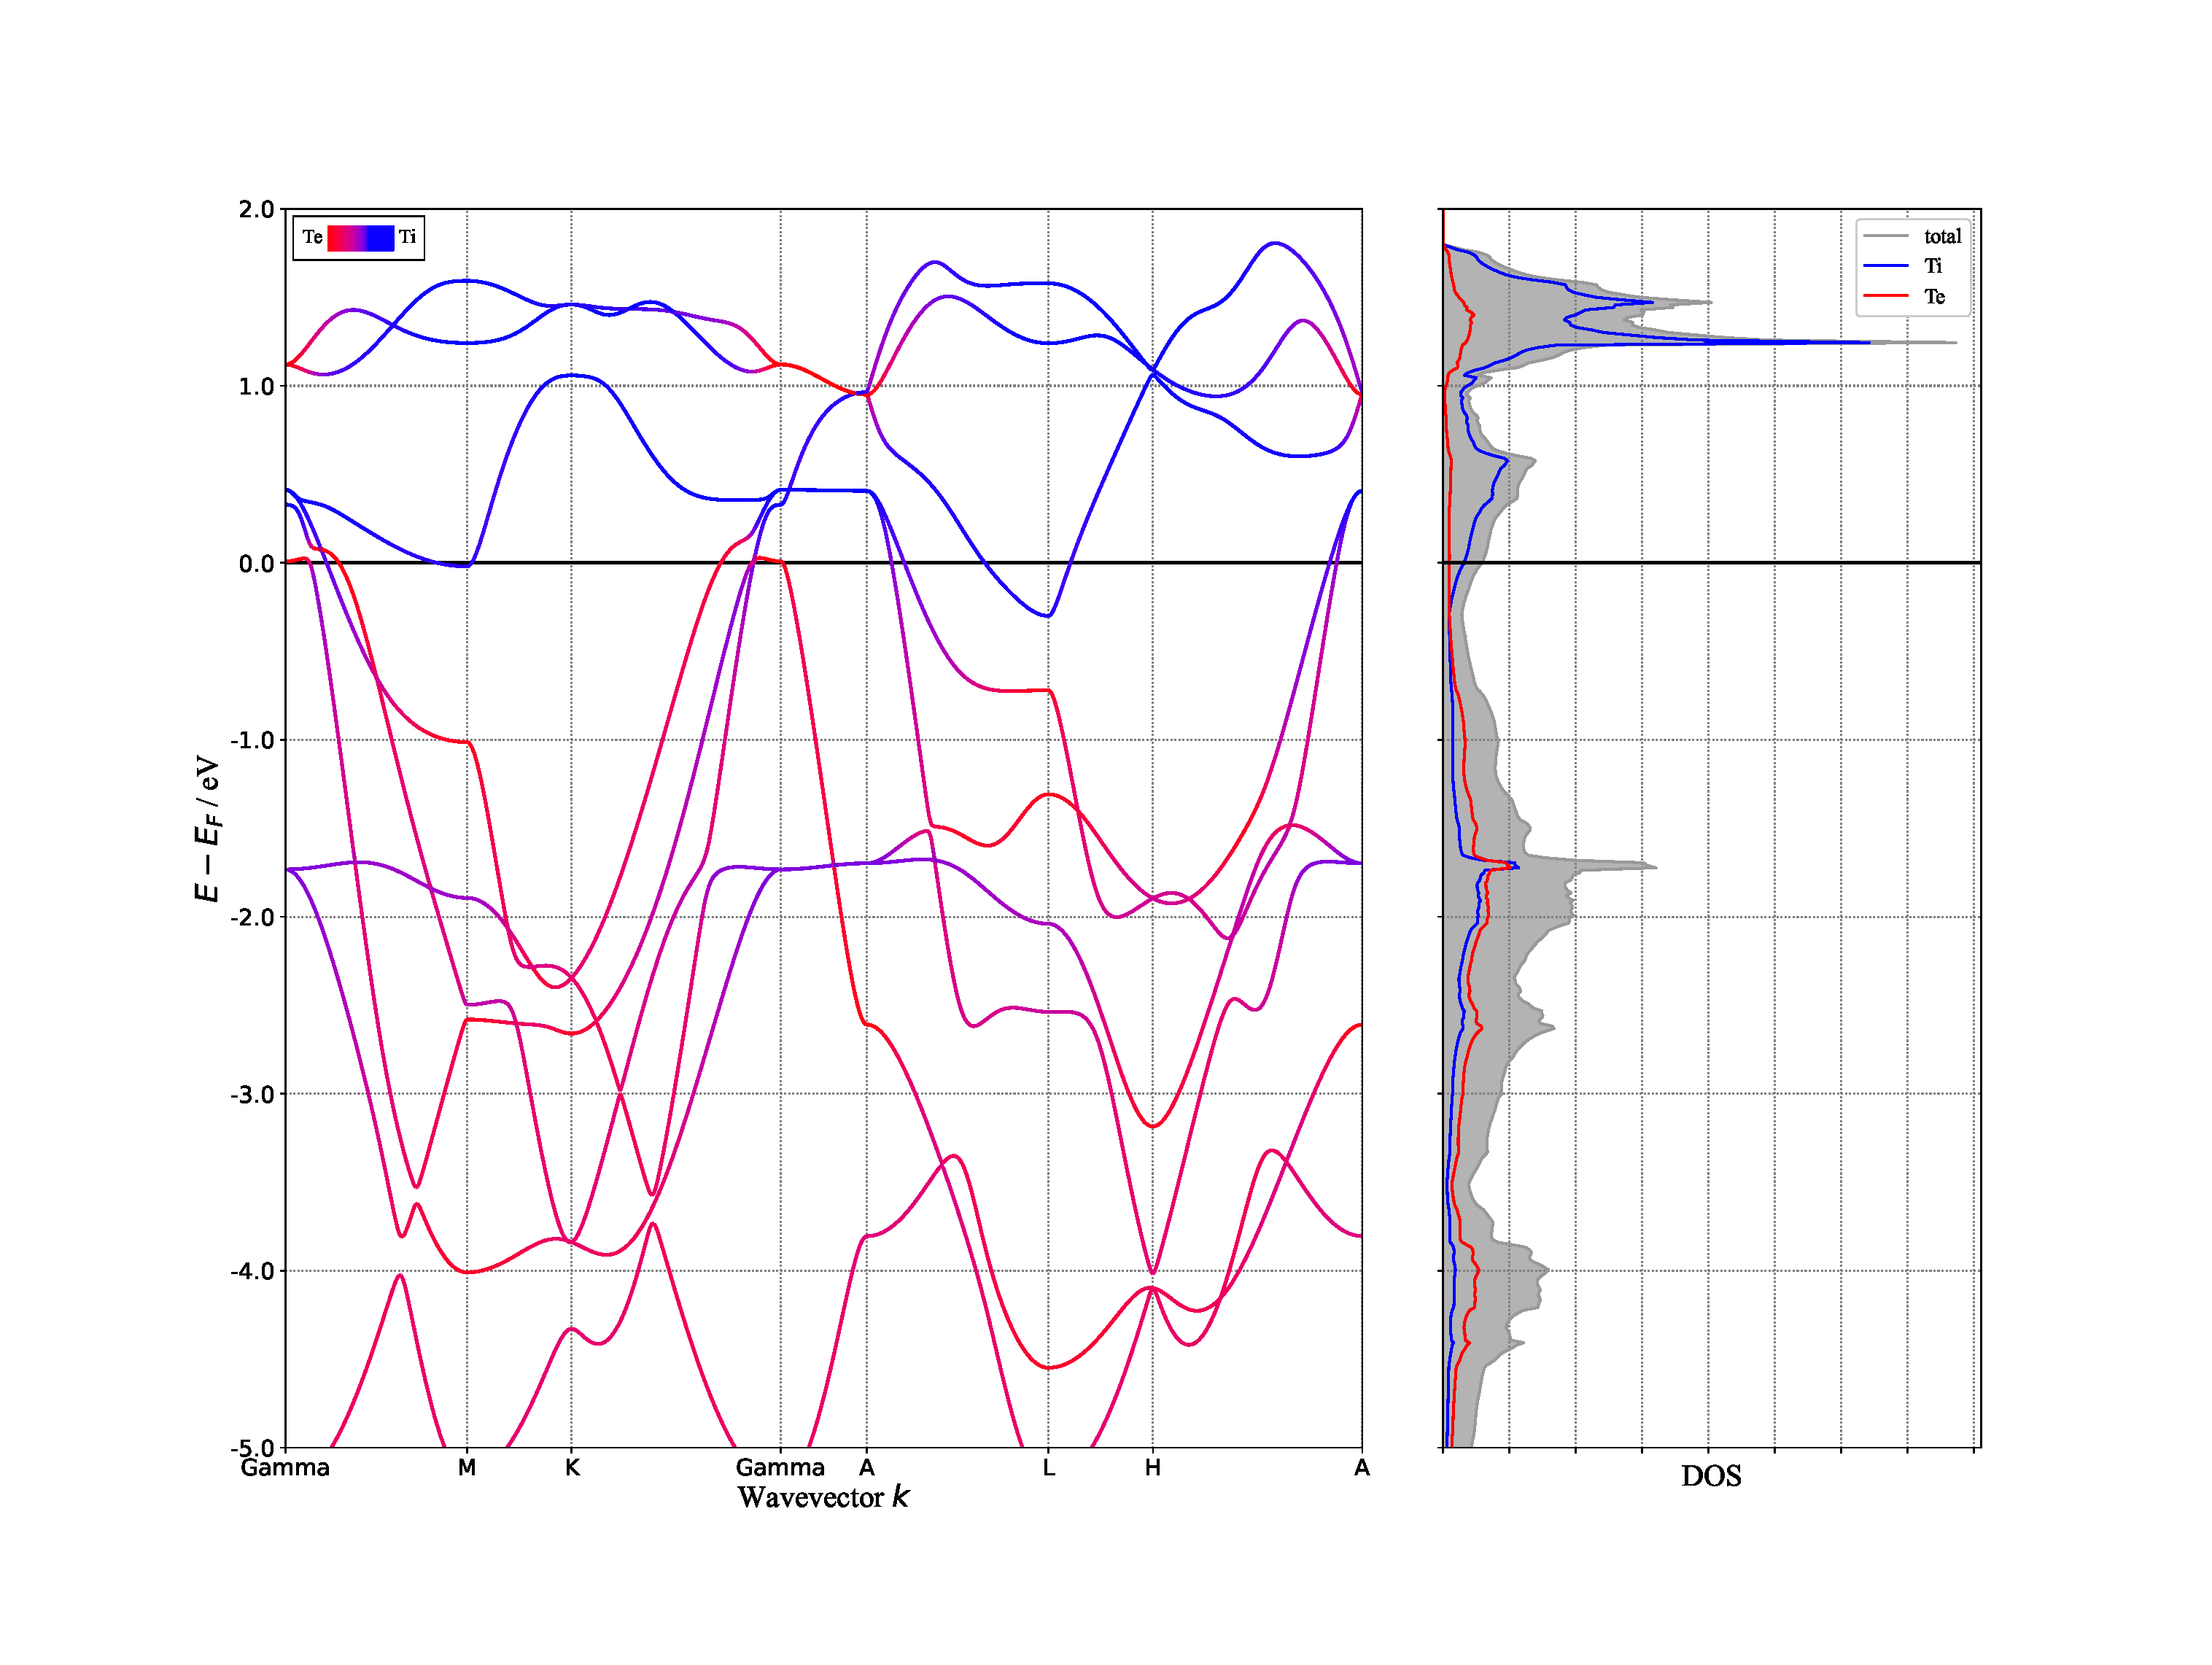
\includegraphics[width=\linewidth]{img/results/TiTe2_SCAN_relaxed_BAND+DOS}
    	\caption{
    	TiTe2}
	\end{subfigure}
\caption{Електронна будова TiS$_2$, TiSe$_2$, TiTe$_2$ червоним кольором позначено вклад атомів халькогену (S, Se, Te) синім атомів металу (Ti), розрахована з SCAN.}
\label{fig:bandstructireSCAN}
\end{figure}

Для того щоб показати наскільки матеріал сильно корельований ми за референс брали саме TiS$_2$ сполуку, закріпляли координати атомів елементарної комірки та варіювали U до 3.0 еВ див. рис. \ref{fig:variationU_GGA}. 

\begin{figure}
	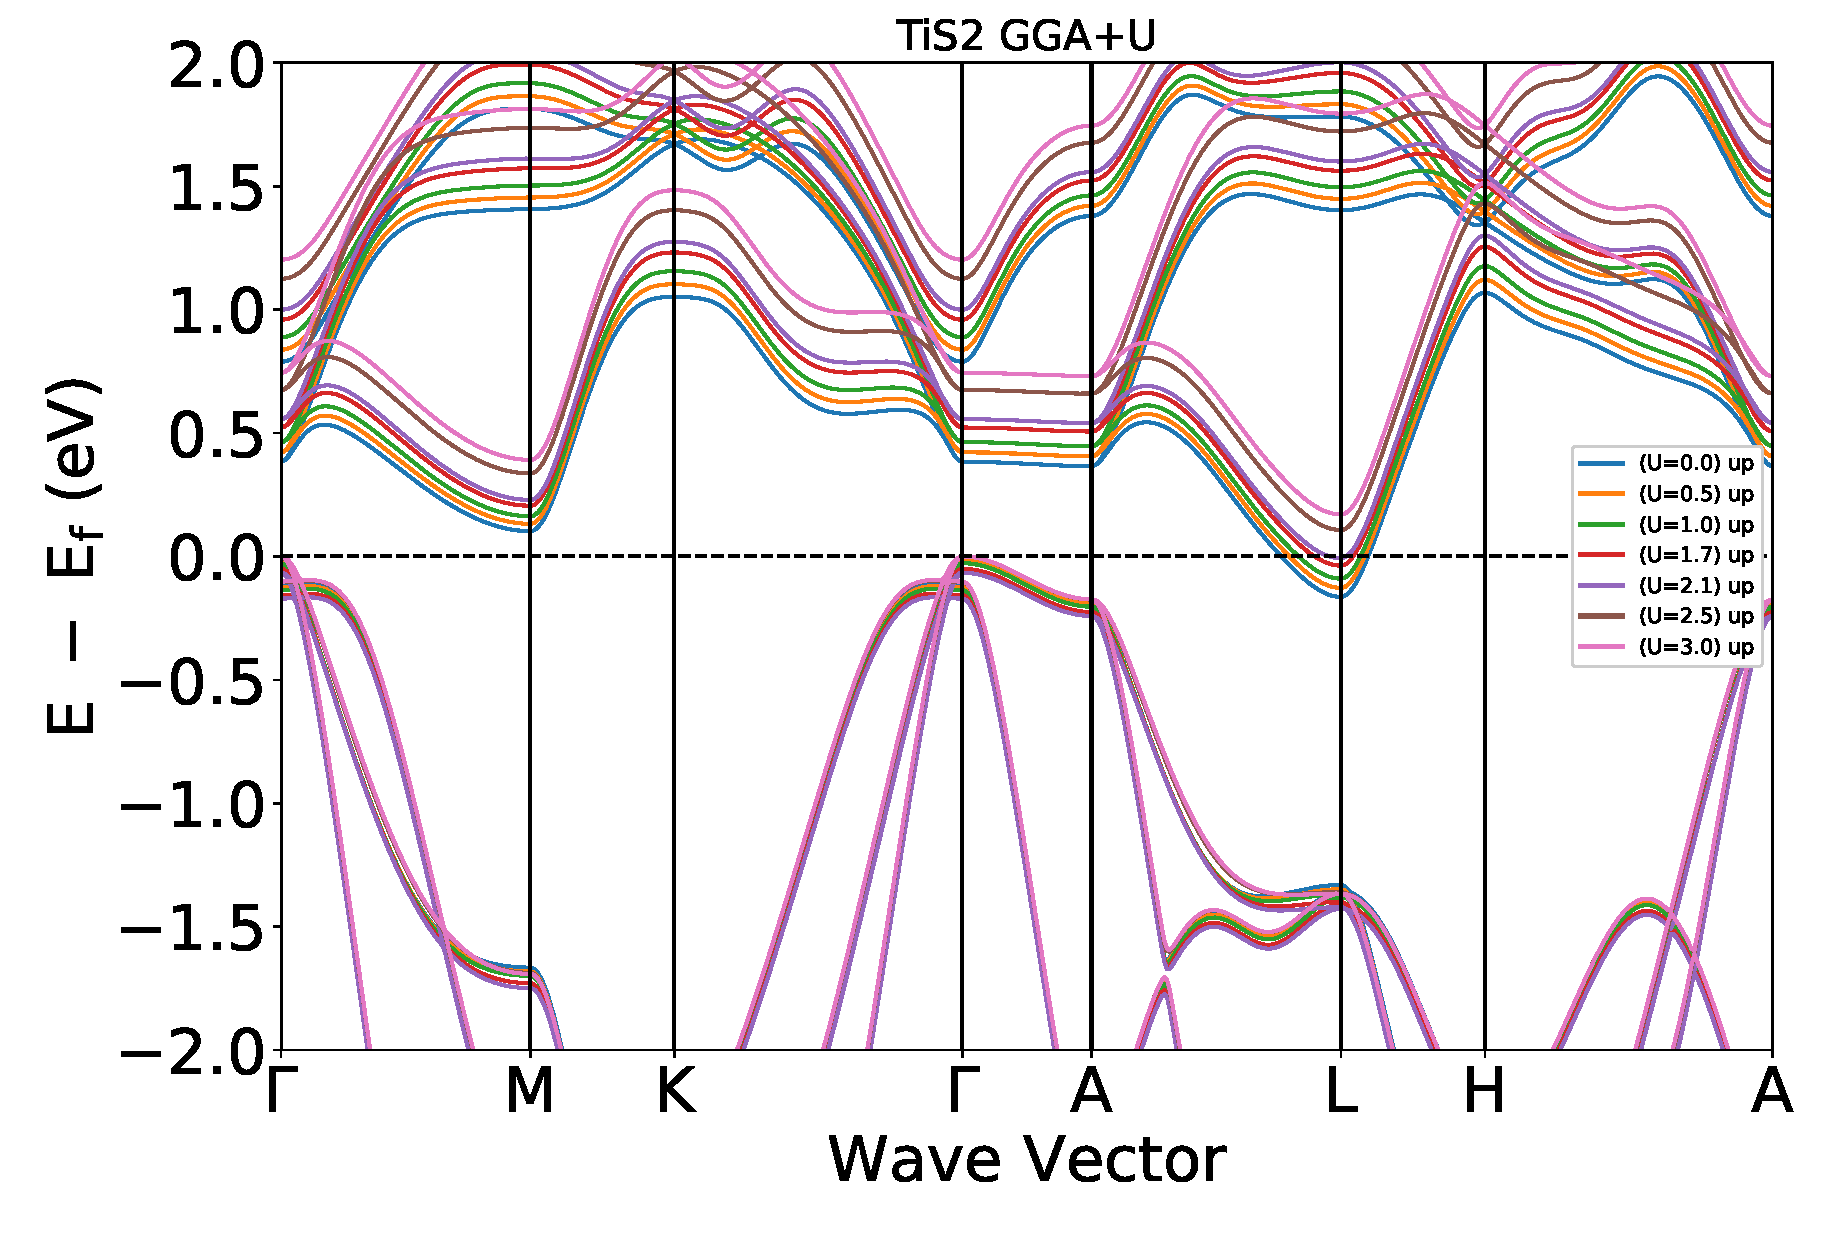
\includegraphics[scale=0.6]{results/TiS2_GGA+U--variation.eps}
	\caption{Зонна структура при варіації U від 0 до 3.0 eV, для TiS$_2$.}
	\label{fig:variationU_GGA}
\end{figure}

Як зазначалось у попередніх розділах, для опису сильнокорельованих систем ми маємо використовувати DFT+U. При прикладених U зонна щілина відкривається таб. \ref{tab:VariationU} на 0.0129 еВ при $U=1.7$ та 0.0587 еВ при $U=2.1$, але цього недостатньо, щоб чітко стверджувати, ща ми маємо напівпровідникову поведінку матеріалу. 

\begin{table}[H]\centering
\scriptsize
\begin{tabular}{lrr}\toprule
\multicolumn{2}{c}{\textbf{Варіація U }} \\\midrule
\multirow{2}{*}{\textbf{U}} &\multirow{2}{*}{\textbf{Band Gap}} \\
& \\
0.0 & -0.1609 \\
0.5 &-0.1134 \\
1.0 &-0.0631 \\
1.7 &0.0129 \\
2.1 &0.0587 \\
2.5 &0.1067 \\
3.0 &0.1699 \\
\bottomrule
\end{tabular}
\caption{Перетин $p$ орбіталей у точці $L$ з варіацією U для TiS$_2$.}\label{tab:VariationU}
\end{table}

Також з даного малюнку можна сказати те, що при збільшені $U=2.5, 3.0$ еВ ми бачимо, як щілина збільшується між $\Gamma$ та $L$ точками. Та при нескінченному збільшені $U$ ми можемо отримати майже будь-яку ширину забороненої зони, але в цей момент постає питання, наскільки адекватна структура комірки буде описуватись? При збільшені $U$ ми будемо мати збільшення напруження в решітці і фактично ми вже будемо розраховувати "інший" зразок. До таких самих висновків приходять для схожого матеріалу TiO$_2$ \cite{doi:10.1063/1.3617244}. Тому ми обираємо $U=2.1$ eV для наступних розрахунків.

\begin{figure}[H]
	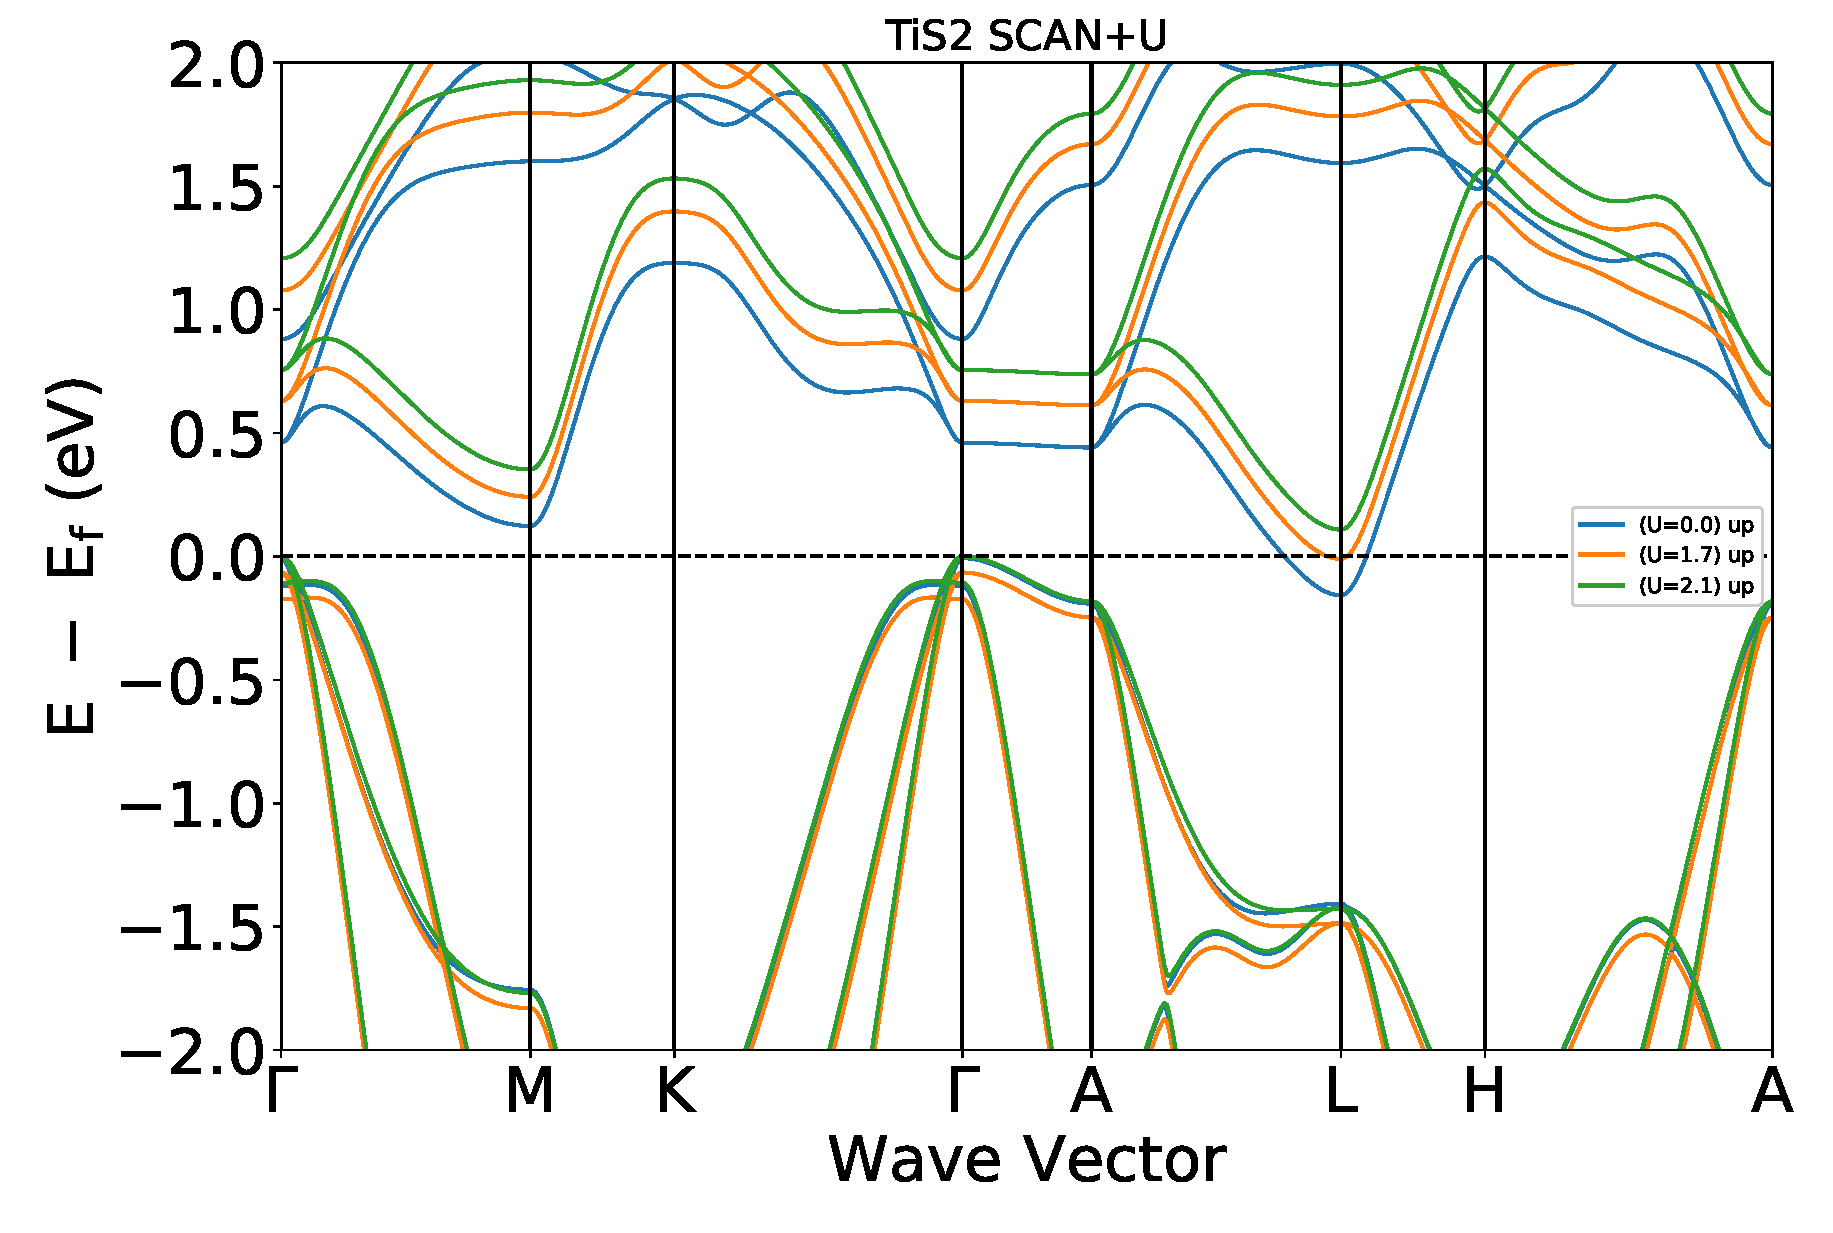
\includegraphics[scale=0.6]{results/TiS2_SCAN+U-variation.eps}
	\caption{Електронна будова TiS$_2$ SCAN + U (U = 0, 1.7, 2.1).}\label{fig:SCAN+U_1.7_2.1}
\end{figure}

Варіюючи U зі значеннями 1.7 еВ, 2.1 еВ рис. \ref{fig:SCAN+U_1.7_2.1} ми отримуємо щілину при таких самих значеннях, що і при GGA+U, але розмір цієї щілини на відміно від GGA PBE, вже узгоджується з розрахунками іншими методами та експериментами. При використанні функціоналу SCAN+U (U = 2.1 eV) ми бачимо, як відкривається зонна щілина порядку $\approx$ 0.1 eV у сполуці TiS$_2$ див. рис. \ref{fig:SCAN+U_tis2}, але цього не відбувається у TiSe$_2$, TiTe$_2$ див. рис. \ref{fig:SCAN+U_tise2}, \ref{fig:SCAN+U_tite2} і це узгоджується з експериментальними даними.

\begin{figure}[H]
	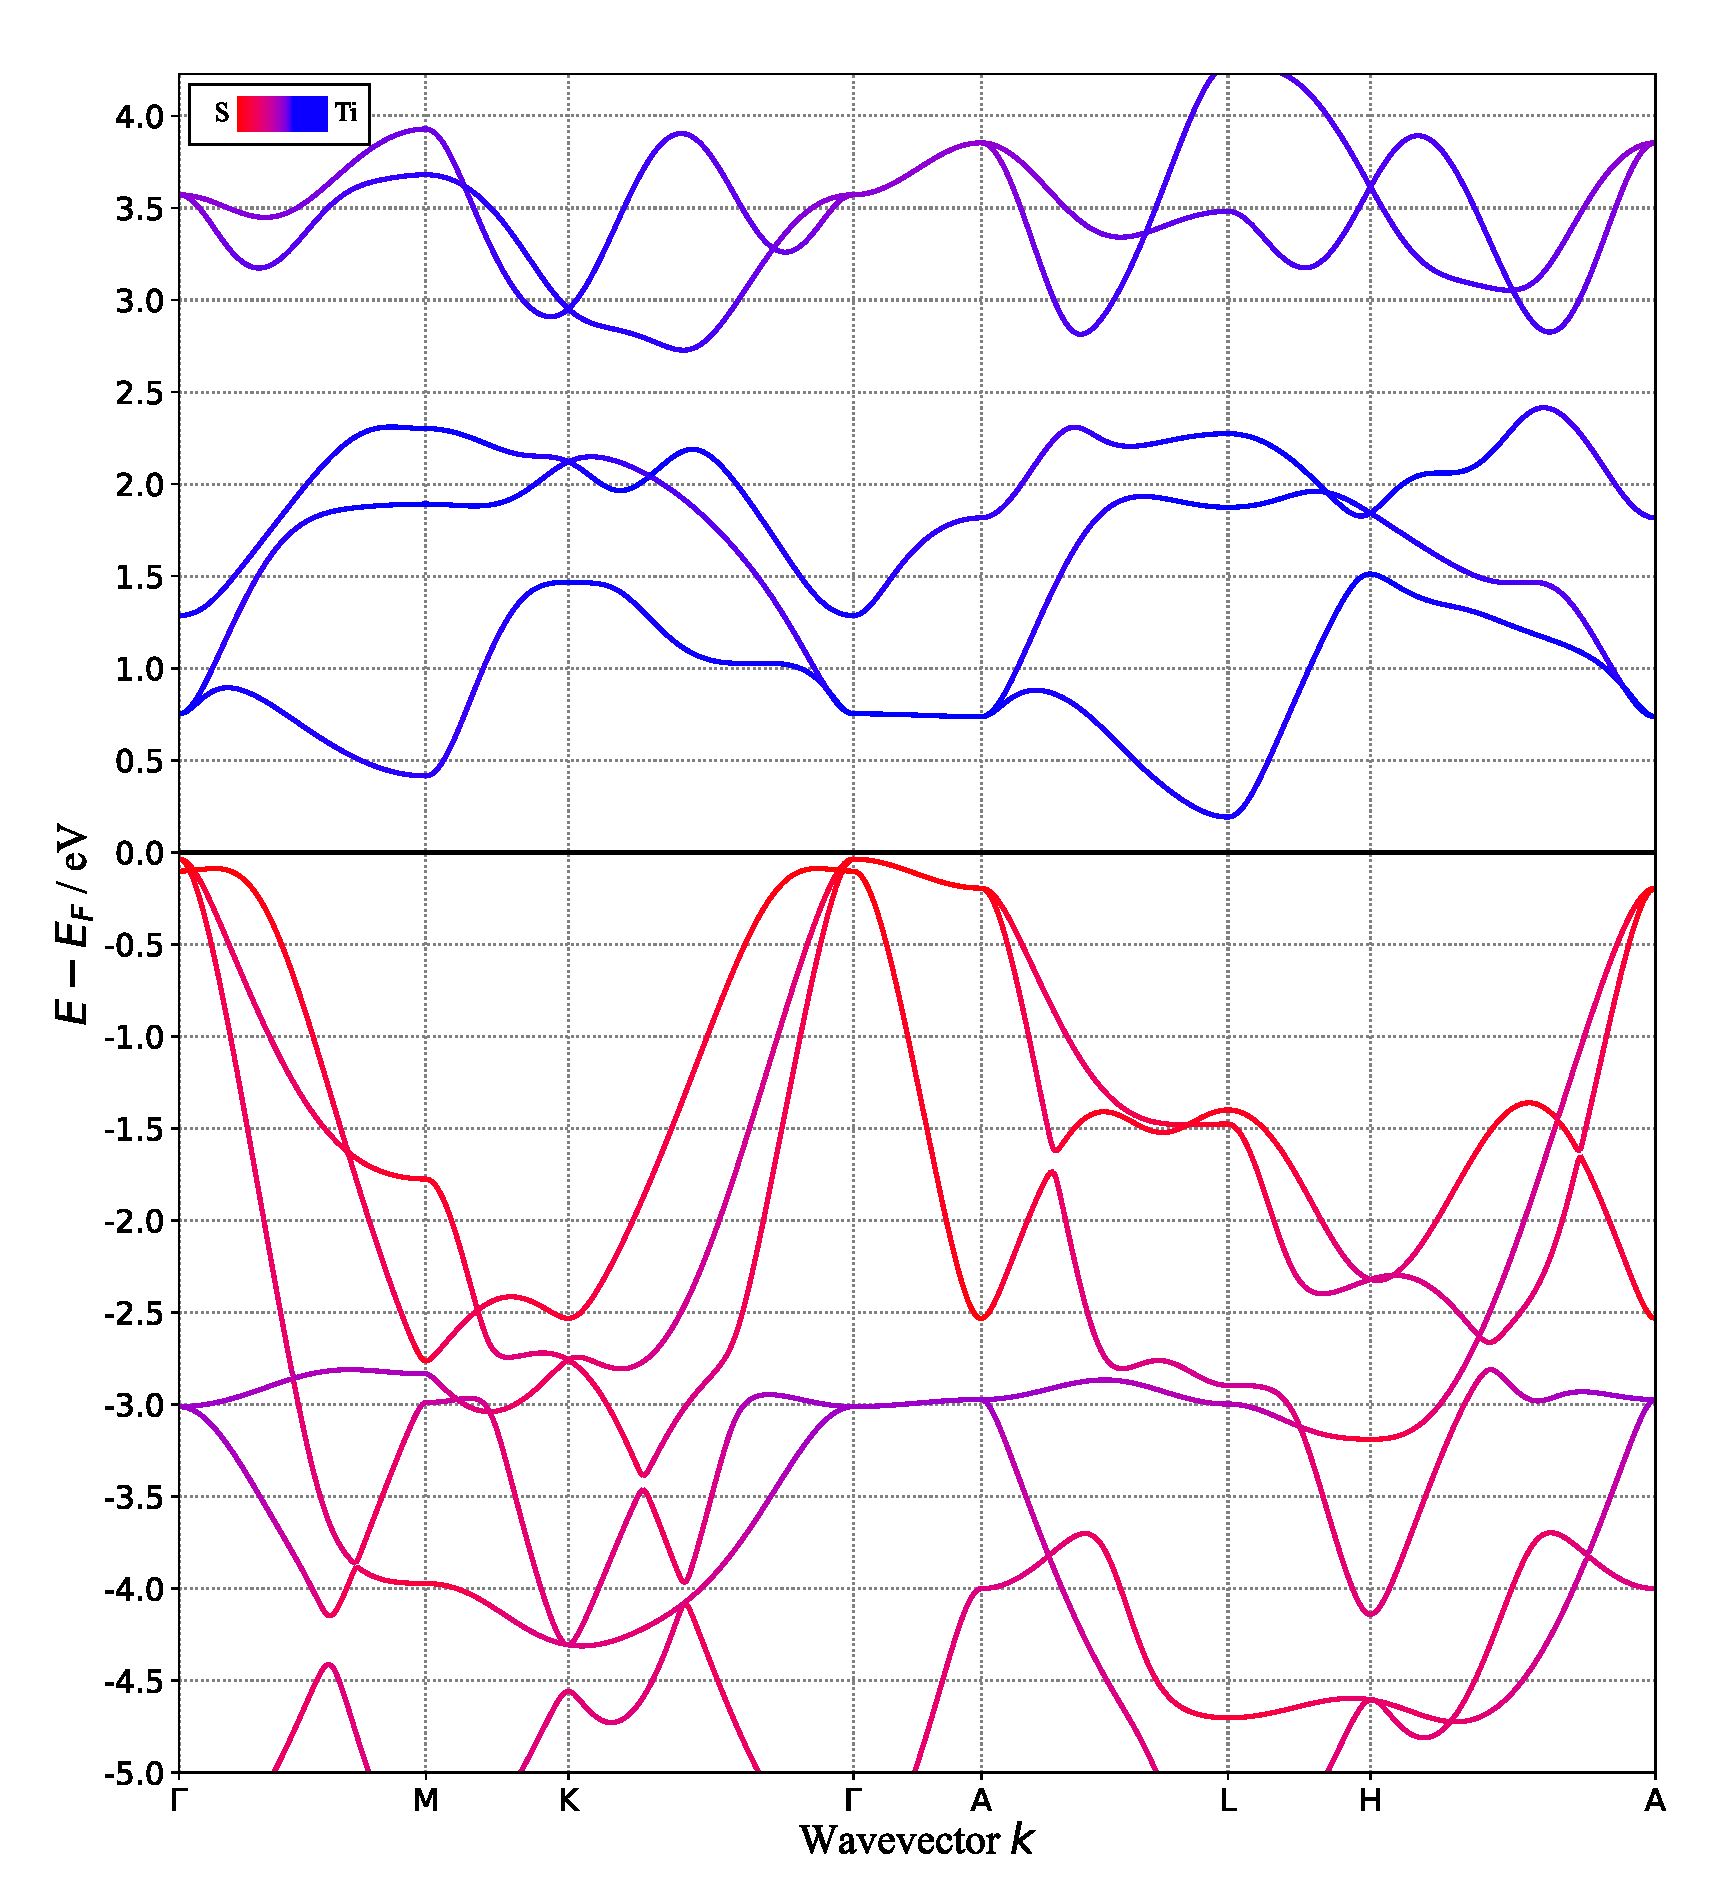
\includegraphics[scale=0.6]{results/SCAN-rVV10+U}
	\caption{Електронна будова TiS$_2$ з використанням поправок rVV10.}\label{fig:rVV10+U}
\end{figure}

Після цього було використано для структурної релаксації вандервальсовські поправки \cite{Peng_2016}, які більш краще описують геометрію решітки та отримати вже наближене до експериментального значення розмір щілини $\approx$ 0.22 eV. див. рис. \ref{fig:rVV10+U}.

\begin{figure}
	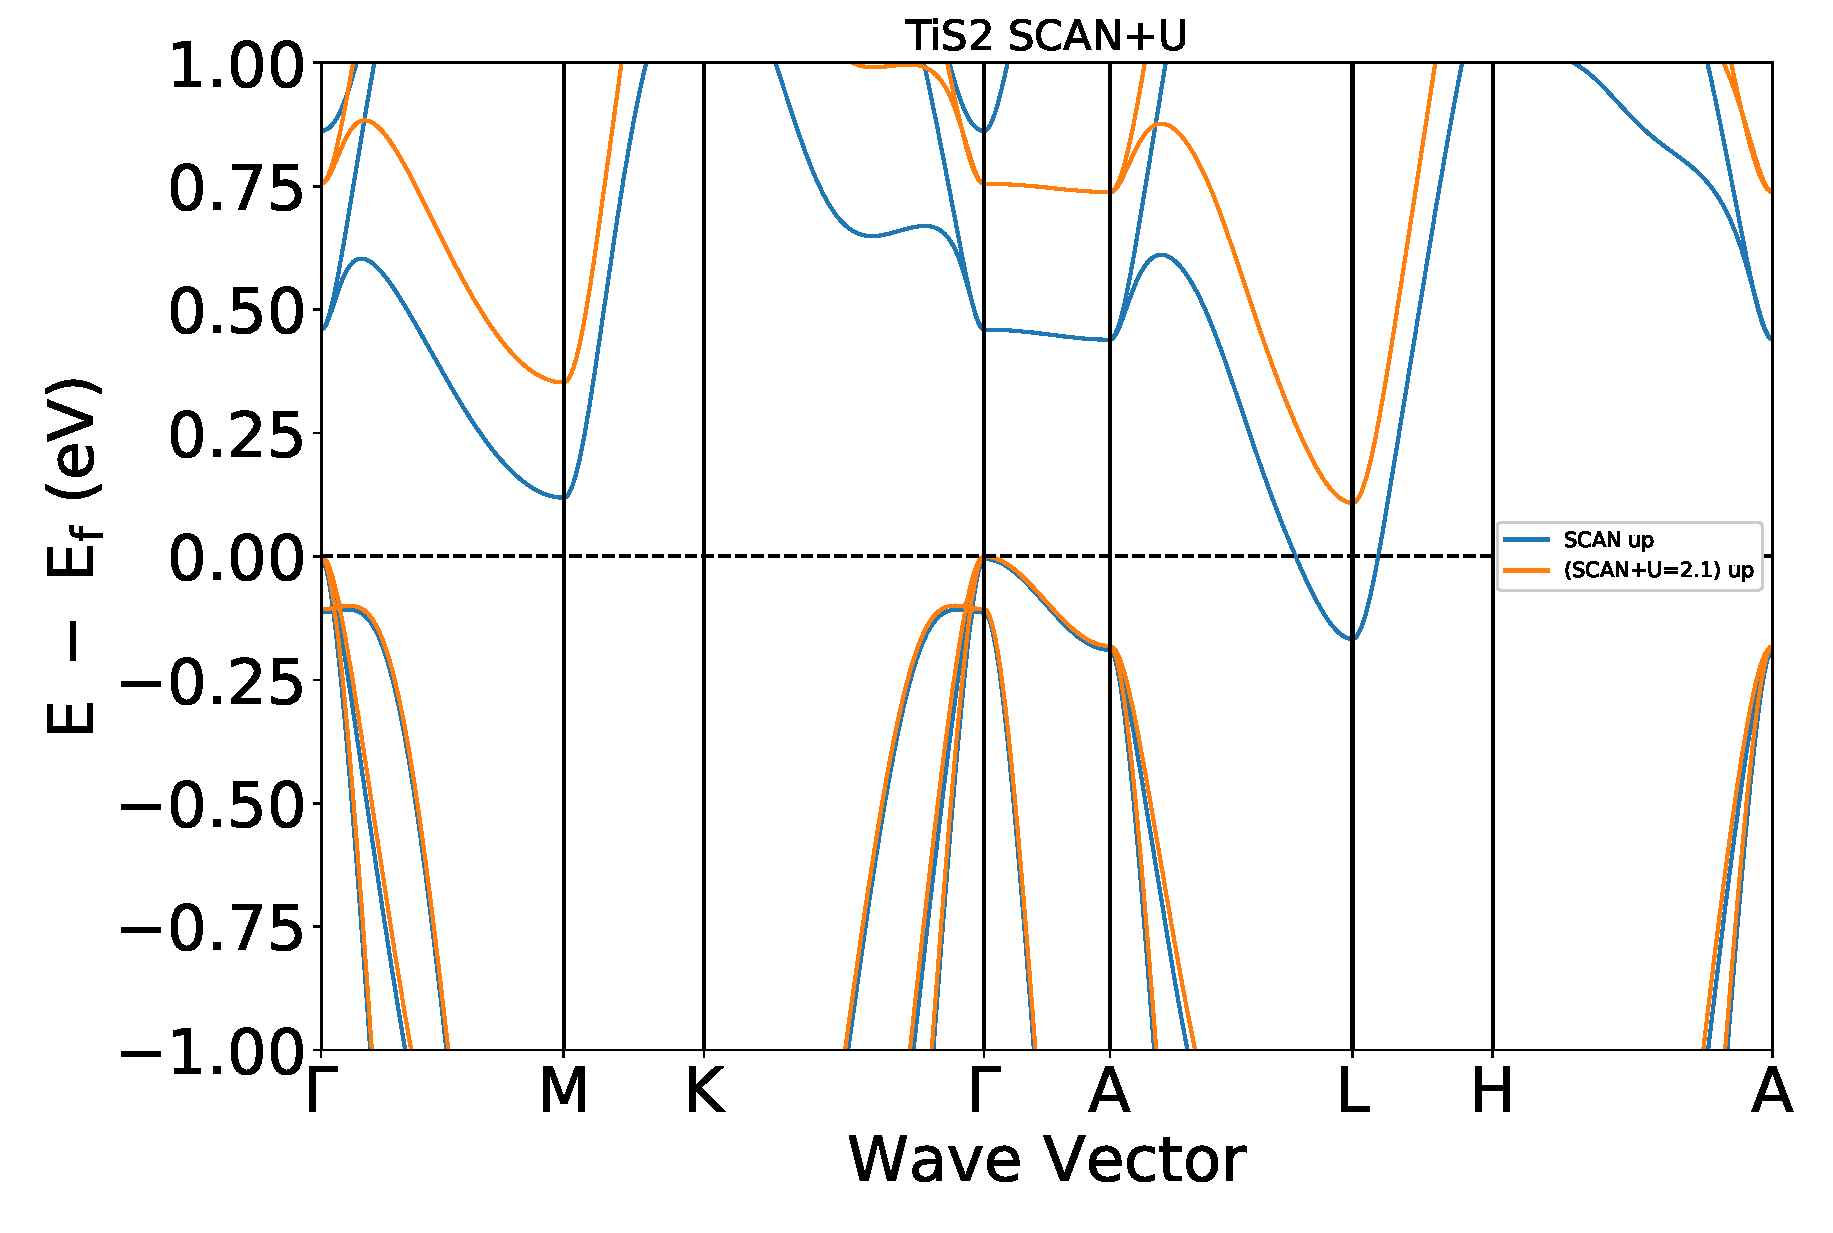
\includegraphics[scale=0.6]{results/TiS2_SCAN_vs._SCAN+U.eps}
	\caption{Електрона будова TiS$_2$ SCAN + U (U = 2.1).}\label{fig:SCAN+U_tis2}
\end{figure}

\begin{figure}
	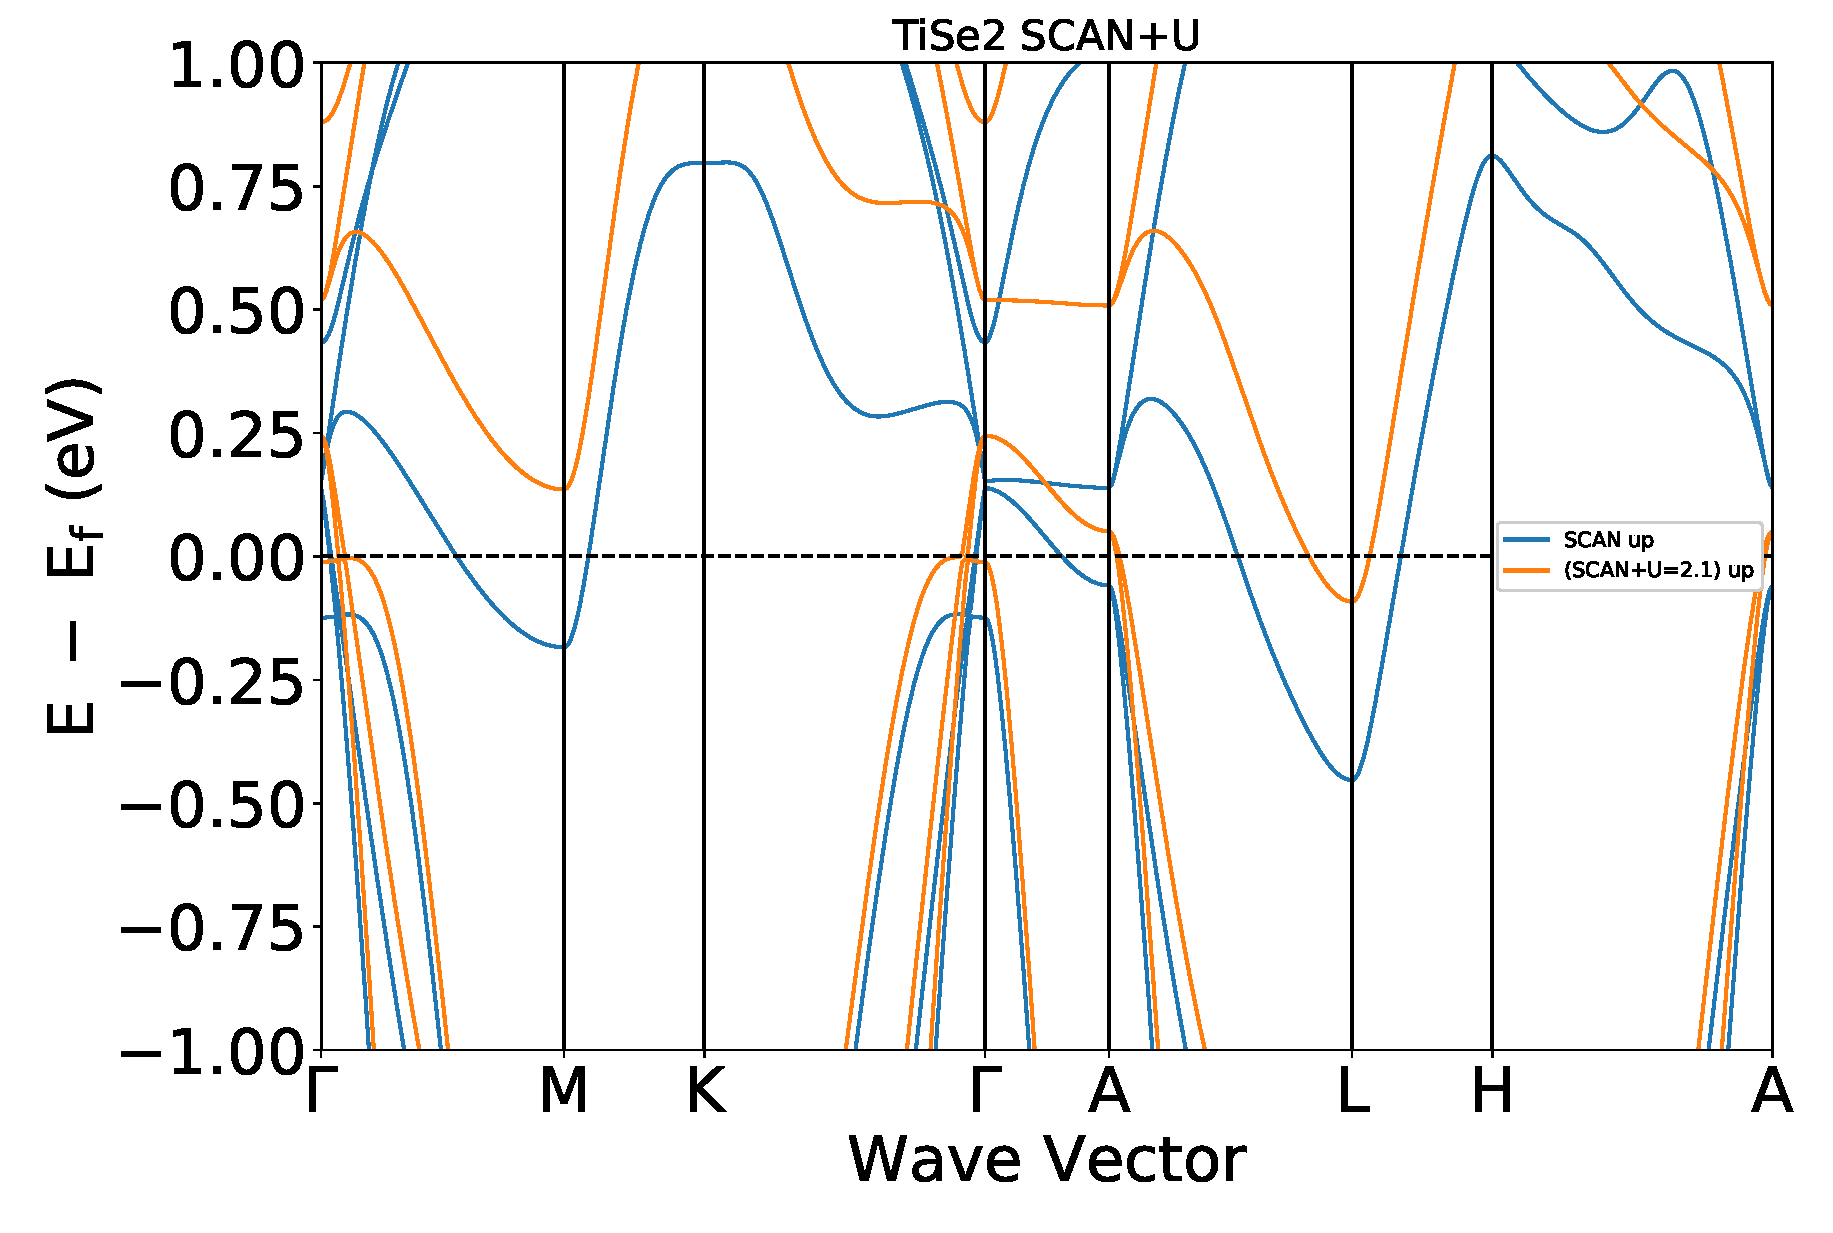
\includegraphics[scale=0.6]{results/TiSe2_SCAN_vs._SCAN+U.eps}
	\caption{Електрона будова TiSe$_2$ SCAN + U (U = 2.1).}\label{fig:SCAN+U_tise2}
\end{figure}

\begin{figure}
	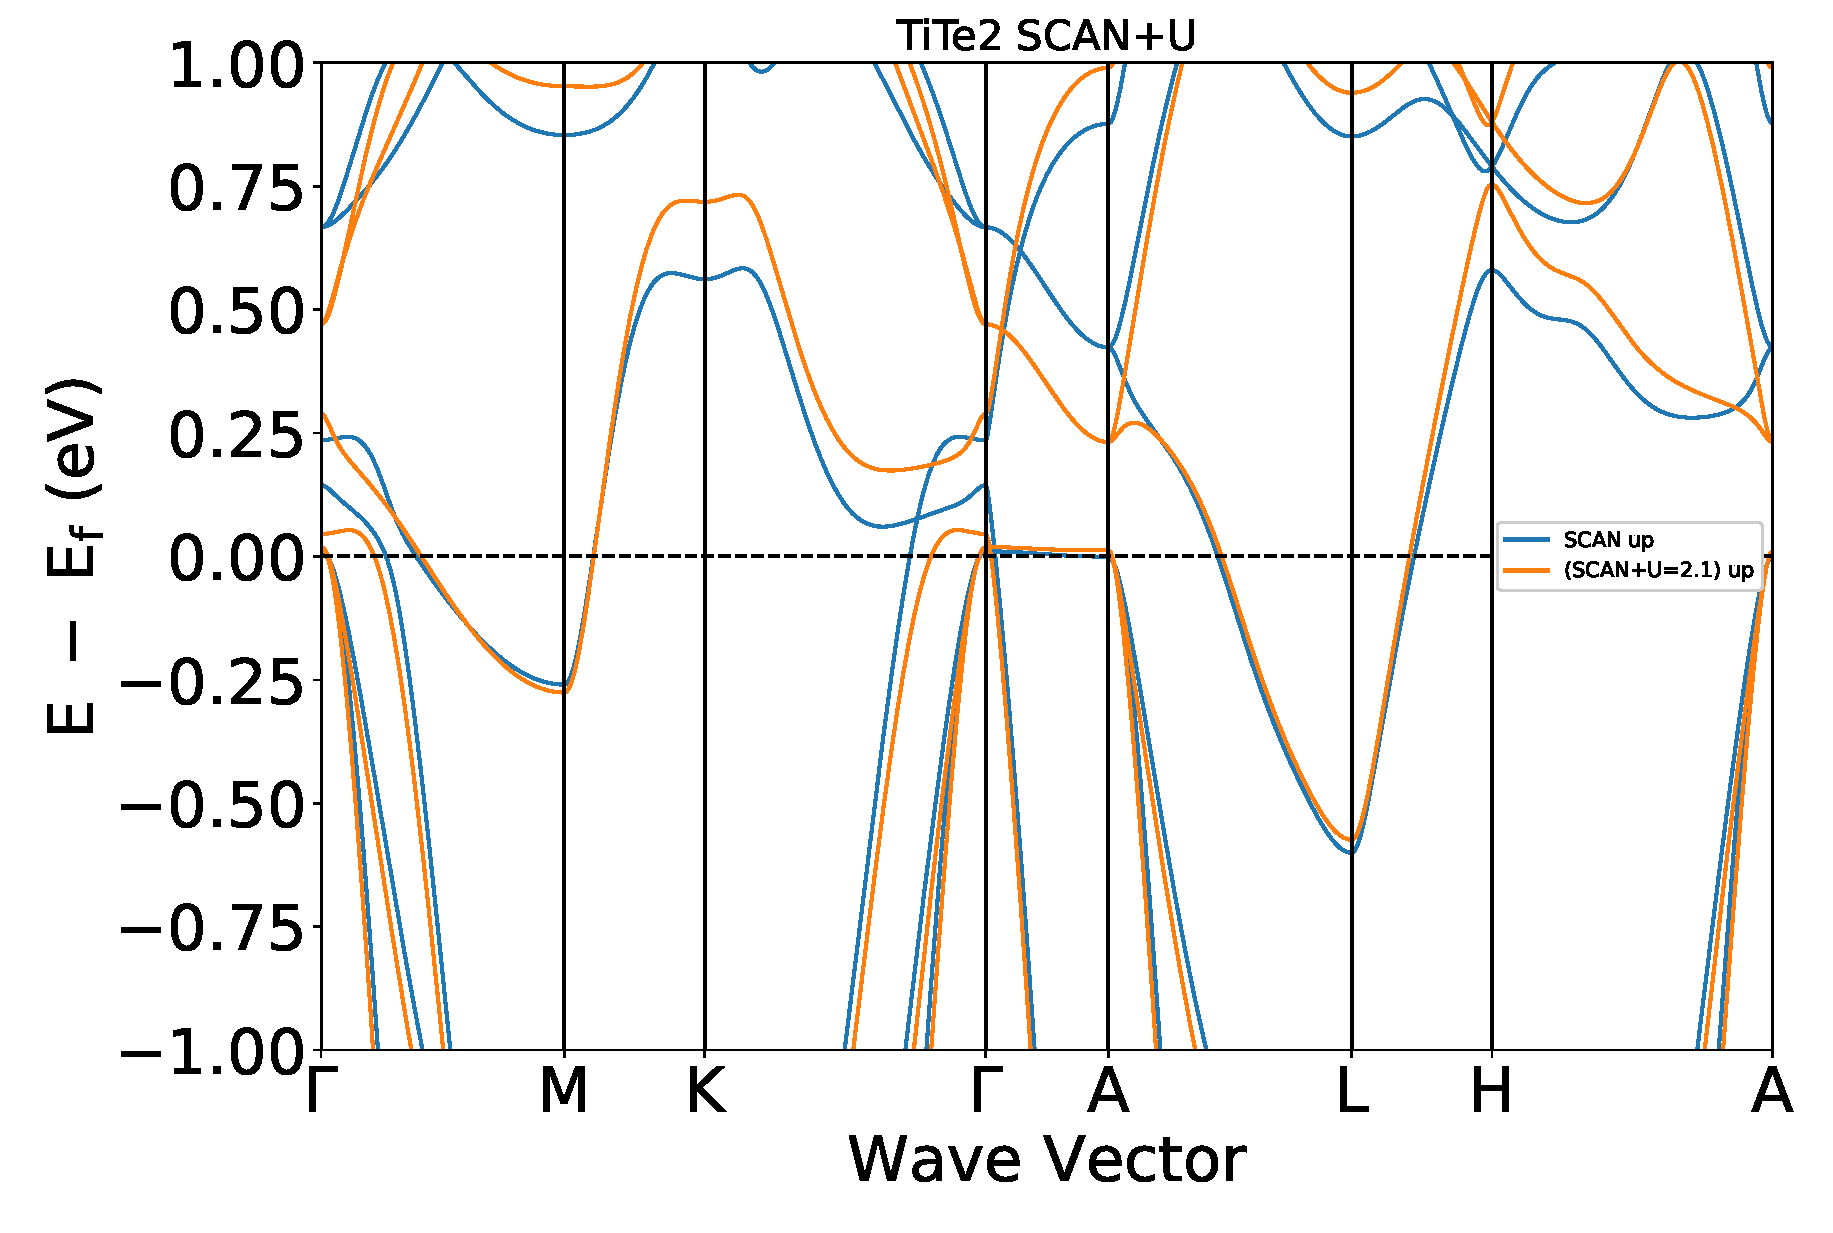
\includegraphics[scale=0.6]{results/TiTe2_SCAN_vs._SCAN+U.eps}
	\caption{Електрона будова TiTe$_2$ SCAN + U (U = 2.1).}\label{fig:SCAN+U_tite2}
\end{figure}

\section{Висновки до розділу}
У останньому розділі були представлені результати ТФГ розрахунків у SCAN наближені. Був проведений аналіз розрахунків, побудовані зони спектри та наведені таблиці постійних ґраток в порівнянні з PBE GGA функціоналом. Виявлені оптимальні значення параметра U, встановлено що U дорівнює 2.1 eV для відкриття енергетичної щілини. 